\documentclass[11pt]{article}

\usepackage[margin=1in]{geometry}
\usepackage{graphicx}
\usepackage{booktabs}
\usepackage{longtable}
\usepackage{array}
\usepackage{amsmath,amssymb}
\usepackage{hyperref}
\usepackage{xcolor}
\usepackage{enumitem}
\usepackage{float}
\usepackage{placeins}
\usepackage{subcaption}
\usepackage{caption}
\usepackage{listings}
\usepackage{microtype}

\hypersetup{
  colorlinks=true,
  linkcolor=blue!50!black,
  citecolor=blue!50!black,
  urlcolor=blue!50!black
}

\lstset{
  basicstyle=\ttfamily\small,
  breaklines=true,
  frame=single,
  columns=fullflexible
}

\newcommand{\ddx}{\textsc{DDXPlus}}
\newcommand{\mlp}{\textsc{MLP}}
\newcommand{\llm}{\textsc{LLM}}
\newcommand{\todo}[1]{\textcolor{red}{#1}}

\title{\textbf{Evidence-Efficient Diagnostic Workup on DDXPlus}\\
\large A Ledger-Controlled Sequential Diagnostic System with Neural Belief Feedback, Graph/Bayesian Analysis, and Live Confirmation}
\author{Baseline Model Research Project}
\date{Compiled May 9, 2026}

\begin{document}
\maketitle

\begin{abstract}
This project studies automatic differential diagnosis under incomplete evidence. Rather than treating diagnosis as a static classification problem, we model it as a sequential workup: an agent begins with only the initially visible \ddx{} evidence, requests additional evidence fields under a deterministic ledger, updates diagnostic belief, and stops when the case appears sufficiently resolved. The final defended method is Notebook 13: a single \llm{} evidence-acquisition controller paired with a BASD-style partial-evidence \mlp{} that supplies confidence, margin, entropy, agreement, and stopping signals. On the frozen 49-case live confirmation, this system reaches $43/49 = 0.878$ top-1 accuracy, $0.918$ top-3, $0.939$ top-5, macro-F1 $0.845$, with only $6.59$ mean evidence requests. A fresh live run of the same base architecture inside Notebook 24 reaches $45/49 = 0.918$ with $6.20$ requests, supporting the robustness of the base method. Offline graph/Bayesian extensions improve saved traces as high as $47/49$, but live confirmation did not promote them; targeted branching similarly recovered some failures but introduced a regression. The strongest supported claim is therefore not unrestricted multi-agent superiority, but evidence-efficient ledger-controlled diagnostic workup with a neural stopping monitor and a clear experimental ladder of positive and negative results.
\end{abstract}

\tableofcontents
\newpage

\section{Executive Summary}

The original ambition was a multi-agent diagnostic workup copilot. The implemented project sharpened this into a more defensible research question:
\begin{quote}
\emph{Can structured sequential evidence acquisition approach full-evidence diagnostic performance while revealing only a small targeted subset of evidence?}
\end{quote}

The final defended system is not a free-form chat agent. It is a controlled workup loop in which a deterministic evidence ledger governs what is visible, what may legally be requested, and how much evidence has been acquired. The \llm{} chooses requests from legal evidence fields, while a partial-evidence \mlp{} estimates whether the visible state is diagnostically resolved. The project includes a complete baseline ladder: initial-evidence neural baseline, full-evidence ceiling, \llm{}-only sequential baseline, matched-evidence classifier, hybrid \llm{}/\mlp{} stopping, graph-ledger ablations, Bayesian value-of-information experiments, calibrated graph/Bayes rescue, and trajectory branching.

\begin{table}[H]
\centering
\caption{Most important final results. ``All fields'' means all \ddx{} structured evidence is visible and is used only as a ceiling comparator.}
\resizebox{\textwidth}{!}{%
\begin{tabular}{lrrrrr}
\toprule
System & Cases & Accuracy & Top-3 & Top-5 & Mean requests \\
\midrule
Initial-evidence MLP, full test split & 134,529 & 0.378 & 0.615 & 0.730 & 0 \\
Full-evidence MLP ceiling, full test split & 134,529 & 0.996 & 1.000 & 1.000 & all fields \\
LLM-only sequential, $\lambda=0.10$ & 24 & 0.917 & 0.917 & 0.917 & 13.04 \\
Selected MLP-stop hybrid, Notebook 13 & 49 & 0.878 & 0.918 & 0.939 & 6.59 \\
Fresh Notebook 13-style base, Notebook 24 & 49 & 0.918 & 0.939 & 0.939 & 6.20 \\
Offline graph/Bayes rescue, Notebook 23 & 49 & 0.959 & -- & -- & 6.96 \\
Live graph/Bayes rescue, Notebook 24 & 49 & 0.918 & 0.939 & 0.939 & 6.39 \\
Live targeted branching, Notebook 27 & 49 & 0.878 & 0.918 & 0.939 & 6.82 selected / 11.45 total \\
MLP-gated confounder branching, Notebook 28 & 49 & 0.898 & 0.959 & 0.959 & 6.63 selected / 9.96 total \\
\bottomrule
\end{tabular}
}
\end{table}

The central scientific story is the gap between sparse initial evidence and complete evidence. A BASD-style \mlp{} gets only $37.8\%$ accuracy when restricted to age, sex, and the official \texttt{INITIAL\_EVIDENCE}; the same style of model reaches $99.6\%$ when all evidence is visible. The diagnostic signal exists, but the difficult problem is deciding which evidence to acquire.

\section{Dataset and Task}

\subsection{DDXPlus}

\ddx{} is a structured synthetic diagnostic dataset introduced for automatic medical diagnosis \cite{ddxplus}. It contains approximately $1.3$ million synthetic patient cases, $49$ pathologies, age, sex, an initial evidence item, a full list of patient evidences, evidence metadata, and differential diagnosis annotations. The evidence schema contains binary, categorical, and multi-choice evidence fields. This makes \ddx{} especially appropriate for sequential workup because the environment can hide all non-initial evidence, then reveal exact structured fields when requested.

In our setup, each patient case is compiled into an episode:
\[
s_0 = (\text{age}, \text{sex}, e_{\text{initial}}),
\]
with a hidden set of evidence roots $E_{\text{hidden}}$. At each turn, the controller may request one legal root evidence field $a_t \in \mathcal{A}(s_t)$ or stop and predict a pathology $d \in \{1,\ldots,49\}$.

\subsection{Why Static Diagnosis Is Not Enough}

The dataset supports two very different tasks:
\begin{enumerate}[leftmargin=*]
    \item \textbf{Static diagnosis}: all available patient evidence is provided, and the model predicts the pathology in one pass.
    \item \textbf{Sequential workup}: only initial evidence is visible, and the model must decide which fields to reveal before predicting.
\end{enumerate}

The full-evidence task is close to solved by strong supervised models, including \ddx{} baselines and later transformer work \cite{ddxplus,ddxt}. Our project therefore does not compete on raw full-information classification. The target is evidence-efficient incomplete-information diagnosis.

\section{Research Grounding and Prior Work}

\subsection{DDXPlus, BASD, and AARLC}

The \ddx{} paper provides both the dataset and the original diagnostic framing \cite{ddxplus}. Two terms from this line of work are especially important for this project:
\begin{itemize}[leftmargin=*]
    \item \textbf{BASD} refers to the supervised neural diagnosis baseline family used in the \ddx{} ecosystem. In practical terms for this project, it means an MLP-style model over a structured observation vector: age, sex, and evidence slots are encoded numerically, and the model predicts a pathology or differential diagnosis. This is why our neural baselines are not bag-of-words text classifiers; they use the official \ddx{} structured evidence schema.
    \item \textbf{AARLC} stands for adaptive alignment of reinforcement learning and classification. It treats automatic diagnosis as two coupled tasks: symptom/evidence inquiry and disease classification. It is important because it argues that an inquiry policy should be aligned with a classifier's diagnostic uncertainty, including entropy and stopping behavior.
\end{itemize}

The BASD family motivates our structured neural representation: age, sex, and evidence slots are encoded into fixed-dimensional vectors with unknown, present, and absent states. AARLC motivates the separation between inquiry and diagnosis \cite{aarlc}. This directly influenced our architecture:
\[
\text{LLM evidence controller} \quad + \quad \text{MLP diagnostic belief head}.
\]

AARLC also supports using classifier entropy as a control signal. In our system, entropy, confidence, and margin from the partial-evidence \mlp{} become stopping criteria rather than merely evaluation diagnostics. We did not implement the full AARLC reinforcement-learning algorithm; instead, we borrowed its key design separation: one component acquires evidence and another component estimates diagnostic belief.

\subsection{Active Feature Acquisition and Cost-Sensitive Diagnosis}

The workup problem is a form of active feature acquisition \cite{afa,costsensitive}. A patient state is a partially observed feature vector; requesting an evidence field reveals a feature at some cost; stopping produces a diagnosis. A simple objective is:
\[
U(\pi) = \mathbb{E}\left[\mathbf{1}\{\hat{y}=y\} - \lambda N_{\text{requests}}\right],
\]
where $\lambda$ is the evidence cost and $N_{\text{requests}}$ is the number of acquired fields. This objective motivated the cost-sensitive \llm{} baseline in Notebook 8 and later evidence-efficiency comparisons.

\subsection{Interactive LLM Diagnosis and Question Asking}

MEDDxAgent is the closest LLM-agent prior work \cite{meddxagent}. It evaluates modular LLM-based differential diagnosis with an orchestrator, history-taking simulator, retrieval, and diagnosis strategy agents. On interactive \ddx{}, MEDDxAgent reports GPT-4o GTPA@1 of about $0.74$ at 5 questions, $0.78$ at 10 questions, and $0.86$ at 15 questions. This prevents overclaiming: LLM agents for \ddx{} workup already exist. Our defensible contribution is narrower: a \ddx{}-native deterministic evidence ledger, BASD-style partial-evidence \mlp{} feedback, matched-evidence evaluation, and extensive ablations.

MediQ and ALFA further motivate our design \cite{mediq,alfa}. They show that asking useful clinical questions is difficult and that confidence/abstention and structured question quality matter. This supports using a model-based stop certificate rather than trusting the \llm{}'s self-confidence alone.

\subsection{Graph and Bayesian Medical Inquiry}

Graph-enhanced medical reasoning systems such as KG4Diagnosis, MedRAG, TriMediQ, and MedKGI show that graph-structured state can constrain diagnosis and improve multi-turn reasoning \cite{kg4diagnosis,medrag,trimediq,medkgi}. MedKGI is particularly close: it combines knowledge graphs, information-guided inquiry, structured records, and hypothesis-driven termination. Our graph work therefore avoids claiming that graph-based diagnosis is new. Instead, it tests a \ddx{}-native graph ledger built from official evidence roots and train-derived disease/evidence statistics.

Bayesian medical inquiry and value-of-information methods motivate the posterior experiments \cite{bayesinquiry,entropytest}. A generic Bayesian workup loop is:
\[
P(D \mid E_t) \propto P(D) \prod_{e \in E_t} P(e \mid D),
\]
\[
\operatorname{VOI}(a \mid E_t) = H(D \mid E_t) - \mathbb{E}_{x \sim P(a \mid E_t)}[H(D \mid E_t, a=x)].
\]
Notebook 19 implements this idea offline. It is mathematically well-grounded, but empirically underperforms the \llm{}-led method because its trajectories become generic and distribution-shifted relative to the partial-evidence \mlp{}.

\section{Problem Formulation}

Let $D$ be a pathology random variable over $49$ classes, and let $X_1,\ldots,X_m$ denote \ddx{} evidence roots. Each case starts with a small visible set $O_0$ containing age, sex, and the initial evidence root. A policy $\pi$ observes $O_t$ and chooses either:
\[
a_t \in \mathcal{A}(O_t) \quad \text{or} \quad \texttt{STOP}.
\]
If $a_t$ is an evidence request, the environment reveals $X_{a_t}$ and appends it to the ledger. If the policy stops, a final head predicts $\hat{D}$.

We evaluate:
\begin{align*}
\text{Accuracy} &= \frac{1}{n}\sum_i \mathbf{1}\{\hat{D}_i = D_i\},\\
\text{Top-}k &= \frac{1}{n}\sum_i \mathbf{1}\{D_i \in \operatorname{TopK}(\hat{p}_i,k)\},\\
\text{Efficiency} &= \mathbb{E}[N_{\text{requests}}],\\
\text{Cost-sensitive utility} &= \text{Accuracy} - \lambda \mathbb{E}[N_{\text{requests}}].
\end{align*}

The key methodological constraint is evidence discipline: the controller cannot inspect hidden evidence unless it requests it. Full-evidence models are used only as ceiling comparators, not as live policies.

\section{Baseline Ladder}

The project deliberately builds a ladder rather than comparing against a weak baseline.

\begin{longtable}{p{0.12\linewidth} p{0.23\linewidth} p{0.55\linewidth}}
\caption{Sequential development ladder.}\\
\toprule
Stage & Notebook(s) & Role \\
\midrule
\endfirsthead
\toprule
Stage & Notebook(s) & Role \\
\midrule
\endhead
One-shot MLP & 01 & Faithful BASD-style initial-evidence classifier. \\
Early sequential agent & 02--06 & Builds the workup environment, ledger, request legality, and refined prompt policy. \\
Full-evidence ceiling & 07 & Same neural family with all evidence visible; establishes the diagnostic ceiling. \\
Cost-sensitive LLM & 08 & Replaces arbitrary request budgets with $\lambda$-controlled stopping. \\
Matched comparison & 09--10 & Separates evidence acquisition value from final classification by training a partial-evidence MLP. \\
Hybrid MLP feedback & 11--13 & Runs the partial-evidence MLP online and promotes MLP-guided stopping. \\
Shortlist and stop ablations & 14--15 & Tests MLP-guided question selection and stop sensitivity; v2 shortlist is rejected. \\
Graph ledger & 16--18 & Tests MedKGI-style and graph-advisory shortlist policies; both underperform Notebook 13. \\
Bayesian VOI & 19 & Offline posterior/VOI controller; mathematically grounded but negative result. \\
Graph context and critic & 20--22 & Graph context helps ranking; conservative graph critic improves saved trace by one case. \\
Graph/Bayes rescue & 23--24 & Offline rescue reaches 47/49, but live confirmation does not promote the rescue layer. \\
Trajectory branching & 25--28 & Multi-trajectory analysis, live targeted branching, and learned MLP-gated confounder branching; useful gains, not promoted over the defended backbone. \\
\bottomrule
\end{longtable}

\section{Algorithmic Progression Across Notebooks}

The project was intentionally iterative. Each notebook tested one algorithmic hypothesis and either promoted it, rejected it, or used it to motivate the next experiment.

\begin{longtable}{p{0.13\linewidth} p{0.24\linewidth} p{0.50\linewidth}}
\caption{Algorithmic approaches tested across the notebook sequence.}\\
\toprule
Notebook(s) & Algorithmic idea & Outcome and lesson \\
\midrule
\endfirsthead
\toprule
Notebook(s) & Algorithmic idea & Outcome and lesson \\
\midrule
\endhead
01 & BASD-style one-shot MLP & Structured neural baseline from initial evidence only. Accuracy was low enough to show that evidence acquisition matters. \\
02--06 & Sequential LLM workup with deterministic ledger & Built the case episode abstraction, legal evidence reveal, decoded evidence summaries, and anchored diagnosis state. \\
07 & Full-evidence MLP ceiling & Same structured diagnosis family with all evidence visible. Near-ceiling result shows DDXPlus is diagnosable once evidence is known. \\
08 & Cost-sensitive LLM stopping & Replaced fixed budgets with $\lambda$-penalized request cost. Moderate $\lambda$ values preserved accuracy while reducing evidence use. \\
09--10 & Matched-evidence and partial-evidence MLP & Tested whether acquired evidence itself is useful. The partial-evidence MLP became the belief monitor for the hybrid system. \\
11--13 & Online MLP feedback and selected stop confirmation & Promoted the main live method: LLM chooses evidence, MLP supplies stop confidence, margin, and entropy. \\
14--15 & MLP shortlist and stop sensitivity & Direct MLP question control was rejected; stop-threshold analysis clarified hard-case trajectories and drift. \\
16--18 & Train-derived graph ledger and graph shortlists & Graph scores had signal, but hard graph control and advisory graph blending did not beat Notebook 13. \\
19 & Bayesian value-of-information ledger & A principled posterior/VOI controller was negative because it selected generic trajectories and shifted the MLP out of distribution. \\
20--22 & Graph context and graph posterior critic & Graph context improved ranking but not top-1; a conservative final graph critic improved the saved 49-case trace by one case. \\
23--24 & Calibrated graph/Bayes rescue and live confirmation & Offline rescue reached 47/49, but fresh live confirmation did not promote it. \\
25--26 & Base trajectory replicates and offline branching lab & Showed that majority vote is not enough, but selective branching has an oracle and diagnostic ceiling near 47/49. \\
27 & Live targeted branching & Sparse hand-written suspicion trigger recovered two wrong trajectories but introduced one regression; not promoted. \\
28 & Learned MLP-gated confounder graph/Bayes branching & Replaced hand trigger with trained branch gate, added pseudo-candidates and base protection. It improved its live base from 42/49 to 44/49 with zero regressions, but still did not promote over stronger confirmed base runs. \\
\bottomrule
\end{longtable}

\section{Neural Baselines}

\subsection{BASD-Style Evidence Encoding}

The neural baselines use structured \ddx{} observation slots rather than free text. Age is binned, sex is encoded categorically, and each evidence root is represented according to its metadata type. Binary evidence uses present/absent/unknown states; categorical and multi-choice evidence allocate slots for possible values. The state convention follows the BASD style:
\[
x_j =
\begin{cases}
1, & \text{evidence/value present},\\
-1, & \text{evidence explicitly absent},\\
0, & \text{unknown or unrevealed}.
\end{cases}
\]

\subsection{Initial-Evidence MLP}

The assignment baseline is a multilayer perceptron trained on age, sex, and \texttt{INITIAL\_EVIDENCE}. The primary pathology model uses:
\[
h_1=\operatorname{ReLU}(W_1x+b_1), \quad
h_{\ell+1}=\operatorname{ReLU}(W_{\ell+1}h_\ell+b_{\ell+1}),
\]
with hidden sizes $[2048,2048,2048]$ and a final softmax over 49 pathologies:
\[
\hat{p}(D=k\mid x)=\frac{\exp(z_k)}{\sum_{j=1}^{49}\exp(z_j)}.
\]
The primary objective is cross-entropy:
\[
\mathcal{L}_{\text{path}} = -\log \hat{p}(D=y \mid x).
\]
Variants also test soft differential supervision and a joint pathology/differential objective, but the gold-pathology cross-entropy model is the strongest initial-evidence baseline.

\begin{table}[H]
\centering
\caption{Full-test one-shot neural baselines.}
\begin{tabular}{lrrrr}
\toprule
Model & Accuracy & Top-3 & Top-5 & Macro-F1 \\
\midrule
BASD pathology MLP & 0.378 & 0.615 & 0.730 & 0.373 \\
BASD joint MLP & 0.377 & 0.609 & 0.726 & 0.370 \\
BASD differential MLP & 0.319 & 0.518 & 0.628 & 0.294 \\
\bottomrule
\end{tabular}
\end{table}

\subsection{Full-Evidence Ceiling}

Notebook 7 trains the same general neural family with all structured evidence visible. It reaches $0.9958$ test accuracy, top-3/top-5 $1.000$, and macro-F1 $0.9948$. This is not the live task, but it proves that \ddx{} contains enough evidence for near-perfect diagnosis when the relevant fields are known.

\begin{table}[H]
\centering
\caption{Neural baseline ladder.}
\begin{tabular}{lrrrrr}
\toprule
Model & Rows/cases & Evidence & Accuracy & Top-5 & Macro-F1 \\
\midrule
Initial-evidence MLP & 134,529 & Initial only & 0.378 & 0.730 & 0.373 \\
Partial-evidence MLP & 39,998 & Policy-shaped masks & 0.515 & 0.827 & 0.519 \\
Full-evidence MLP & 134,529 & All evidence & 0.996 & 1.000 & 0.995 \\
\bottomrule
\end{tabular}
\end{table}

\section{Deterministic Evidence Ledger}

\subsection{Purpose}

The evidence ledger is the core engineering object. It prevents the system from becoming ``an LLM talking to a dataset.'' The ledger records what is visible, what was requested, how the evidence was decoded, what the diagnosis state was at each turn, and which actions remain legal.

\subsection{State Components}

The implementation uses three conceptual records:
\begin{enumerate}[leftmargin=*]
    \item \textbf{Ledger entry}: turn index, evidence root, question text, source, status, decoded values, and human-readable summary.
    \item \textbf{Diagnosis snapshot}: predicted pathology, ranked differential, confidence, decision, requested field, reasoning, stop signal, deterministic state, and policy flags.
    \item \textbf{Episode state}: case id, split, age, sex, true pathology for evaluation, initial evidence, hidden evidence by root, revealed roots, request history, diagnosis history, shortlist history, and prior differential.
\end{enumerate}

Only the initial evidence root is visible at turn zero. The environment stores the full case, but the agent cannot see it unless it requests a legal root. The update step is deterministic:
\[
O_{t+1} = O_t \cup \{(a_t, x_{a_t})\},
\]
where $x_{a_t}$ is the exact hidden \ddx{} value for the requested root.

\subsection{Legality and Parent-Child Gating}

The ledger enforces:
\begin{itemize}[leftmargin=*]
    \item no duplicate root requests;
    \item child evidence is legal only when the parent evidence is present or implied present;
    \item every reveal is logged with provenance;
    \item diagnosis state must be registered turn by turn.
\end{itemize}

This is clinically and experimentally important. Without legality gating, the agent could ask nonsensical child questions or accidentally use unavailable evidence. Without the ledger, replay and paired evaluation would be much weaker.

\section{Sequential and Cost-Sensitive LLM Baseline}

Notebook 8 uses \texttt{gpt-4.1-mini} as a single evidence-acquisition controller with deterministic API settings. The \llm{} sees the current ledger summary and candidate legal evidence fields, then chooses to request one field or stop. The cost-sensitive rule is governed by an evidence penalty $\lambda$.

\begin{table}[H]
\centering
\caption{Cost-sensitive LLM-only sequential baseline on the 24-case balanced live slice.}
\begin{tabular}{rrrrrr}
\toprule
$\lambda$ & Accuracy & Top-3 & Top-5 & Macro-F1 & Mean requests \\
\midrule
0.10 & 0.917 & 0.917 & 0.917 & 0.846 & 13.04 \\
0.22 & 0.875 & 0.875 & 0.917 & 0.795 & 10.70 \\
0.35 & 0.875 & 0.875 & 0.875 & 0.813 & 8.30 \\
0.50 & 0.417 & 0.625 & 0.750 & 0.274 & 2.20 \\
0.75 & 0.375 & 0.583 & 0.708 & 0.288 & 1.00 \\
\bottomrule
\end{tabular}
\end{table}

This experiment shows a real efficiency frontier. Moderate $\lambda$ values preserve high accuracy while reducing requests; aggressive values stop too early and collapse toward the initial-evidence baseline.

\begin{figure}[H]
\centering
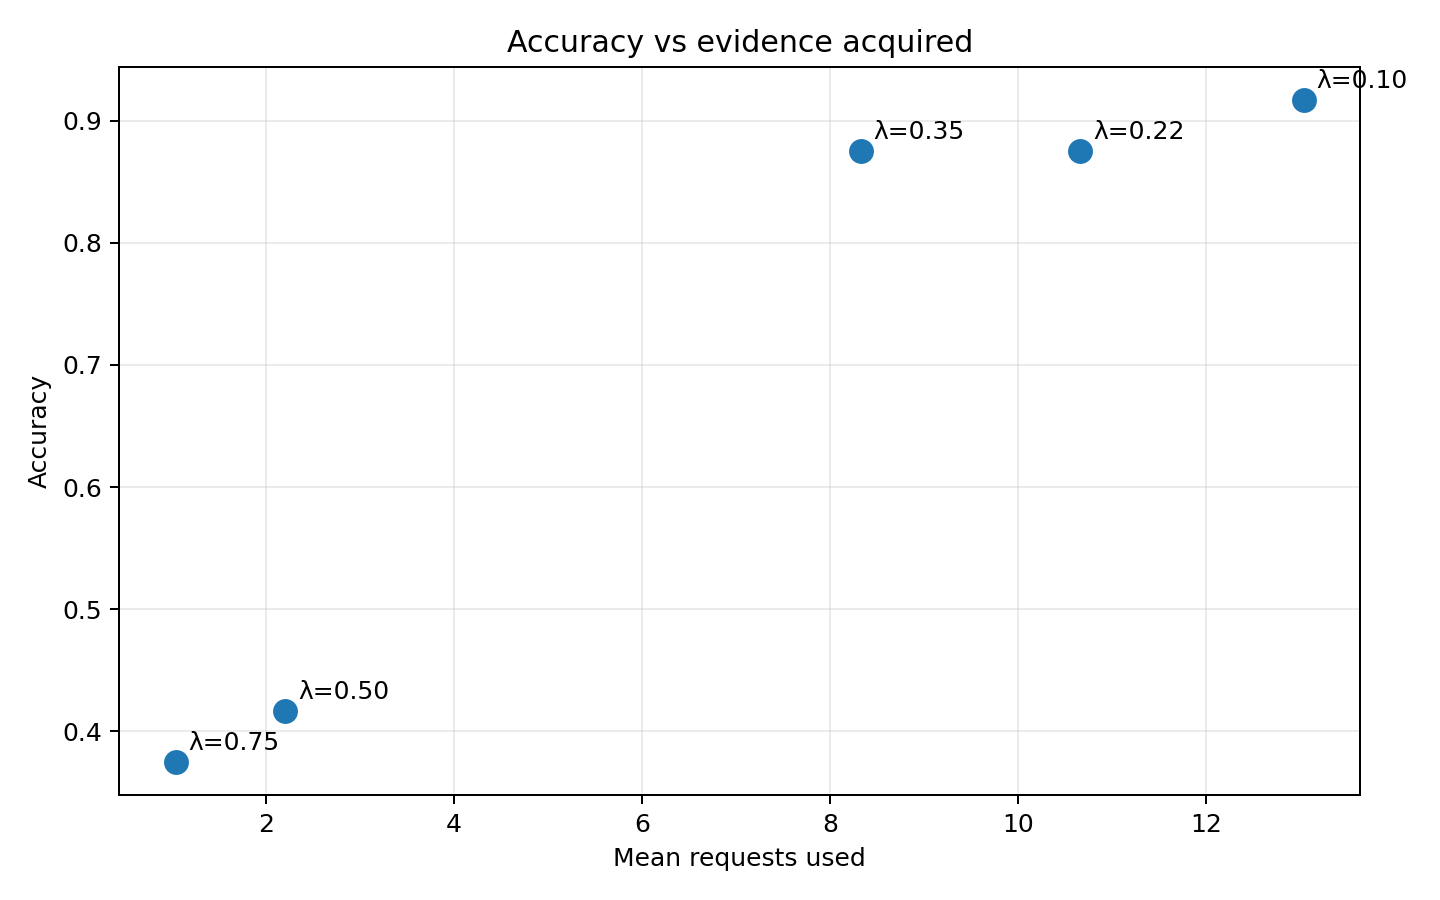
\includegraphics[width=0.82\linewidth]{artifacts/sequential_single_agent_cost_sensitive/single_agent_cost_sensitive_live_test_1perclass_cap24_5lambdas_lambda_cost_24case_wide_sweep_v1/figures/accuracy_vs_mean_requests.png}
\caption{Accuracy versus mean requests for the cost-sensitive \llm{} sequential baseline. The curve identifies the useful region near $\lambda=0.10$--$0.35$ and the failure region at $\lambda \ge 0.50$.}
\end{figure}

\section{Partial-Evidence MLP and Matched-Evidence Evaluation}

Notebook 10 trains a partial-evidence \mlp{} using masks shaped by empirical sequential traces. This model is not intended to replace the \llm{} controller; it is a diagnostic belief head for partially observed states. Its softmax output provides:
\[
p_{\mlp}(D \mid O_t),
\]
plus confidence, margin, entropy, top-k candidates, and agreement with the \llm{}.

The entropy is:
\[
H_{\mlp}(O_t) = -\sum_{d=1}^{49} p_{\mlp}(d\mid O_t)\log p_{\mlp}(d\mid O_t).
\]
The top-1 confidence and margin are:
\[
c_t = \max_d p_{\mlp}(d\mid O_t), \qquad
m_t = p_{\mlp}(d_1\mid O_t) - p_{\mlp}(d_2\mid O_t),
\]
where $d_1$ and $d_2$ are the top two \mlp{} diagnoses.

Matched-evidence evaluation asks whether a direct classifier can diagnose from the same evidence acquired by the sequential policy. This separates two effects:
\[
\text{value} = \text{evidence acquired} + \text{reasoner using that evidence}.
\]
The partial-evidence comparator nearly matches the \llm{} on useful 24-case settings, which is why the final architecture uses the \mlp{} as a belief monitor.

\section{Proposed Method: LLM-Led Workup with MLP-Guided Stopping}

\subsection{Architecture}

The proposed Notebook 13 method has four moving pieces:
\begin{enumerate}[leftmargin=*]
    \item \textbf{Ledger}: deterministic state, legal actions, evidence reveal, request history.
    \item \textbf{LLM controller}: selects the next evidence field or proposes stopping.
    \item \textbf{Partial-evidence MLP}: evaluates the current partial state after every ledger update.
    \item \textbf{Final head}: agreement/conservative hybrid over \llm{} and \mlp{} outputs.
\end{enumerate}

\begin{lstlisting}[caption={Conceptual Notebook 13 loop.}]
initialize ledger with age, sex, INITIAL_EVIDENCE
while request_count < max_cap:
    legal_actions = ledger.legal_actions()
    llm_decision = LLM(ledger_summary, legal_actions, current_differential)
    mlp_state = MLP(encode_visible_ledger(ledger))
    if selected_stop_certificate(llm_decision, mlp_state):
        break
    requested_root = normalize_and_validate(llm_decision.request)
    ledger.reveal(requested_root)
    ledger.register_diagnosis(llm_decision, mlp_state)
return final_head(LLM_final, MLP_final, agreement_state)
\end{lstlisting}

\subsection{Stop Certificate}

Notebook 12 performs an offline replay ablation and selects the stop rule used live in Notebook 13:
\[
\begin{aligned}
N_{\text{requests}} &\ge 1,\\
c_t &\ge 0.70,\\
m_t &\ge 0.20,\\
H_{\mlp}(O_t) &\le 0.10,\\
\text{stability} &\ge 0.
\end{aligned}
\]
This is intentionally conservative: the \llm{} still chooses evidence, but the \mlp{} supplies the main signal that enough evidence has been acquired.

\begin{table}[H]
\centering
\caption{Stopping-policy ablation. The selected MLP-guided policy outperforms pure LLM stopping at a similar request budget.}
\begin{tabular}{llrr}
\toprule
Stop policy & Final head & Accuracy & Mean requests \\
\midrule
Best pure LLM-only stop & LLM & 0.833 & 6.33 \\
Selected MLP-guided stop & Agreement hybrid & 0.917 & 6.88 \\
Best higher-budget MLP final & MLP & 0.958 & 9.80 \\
\bottomrule
\end{tabular}
\end{table}

\begin{figure}[H]
\centering
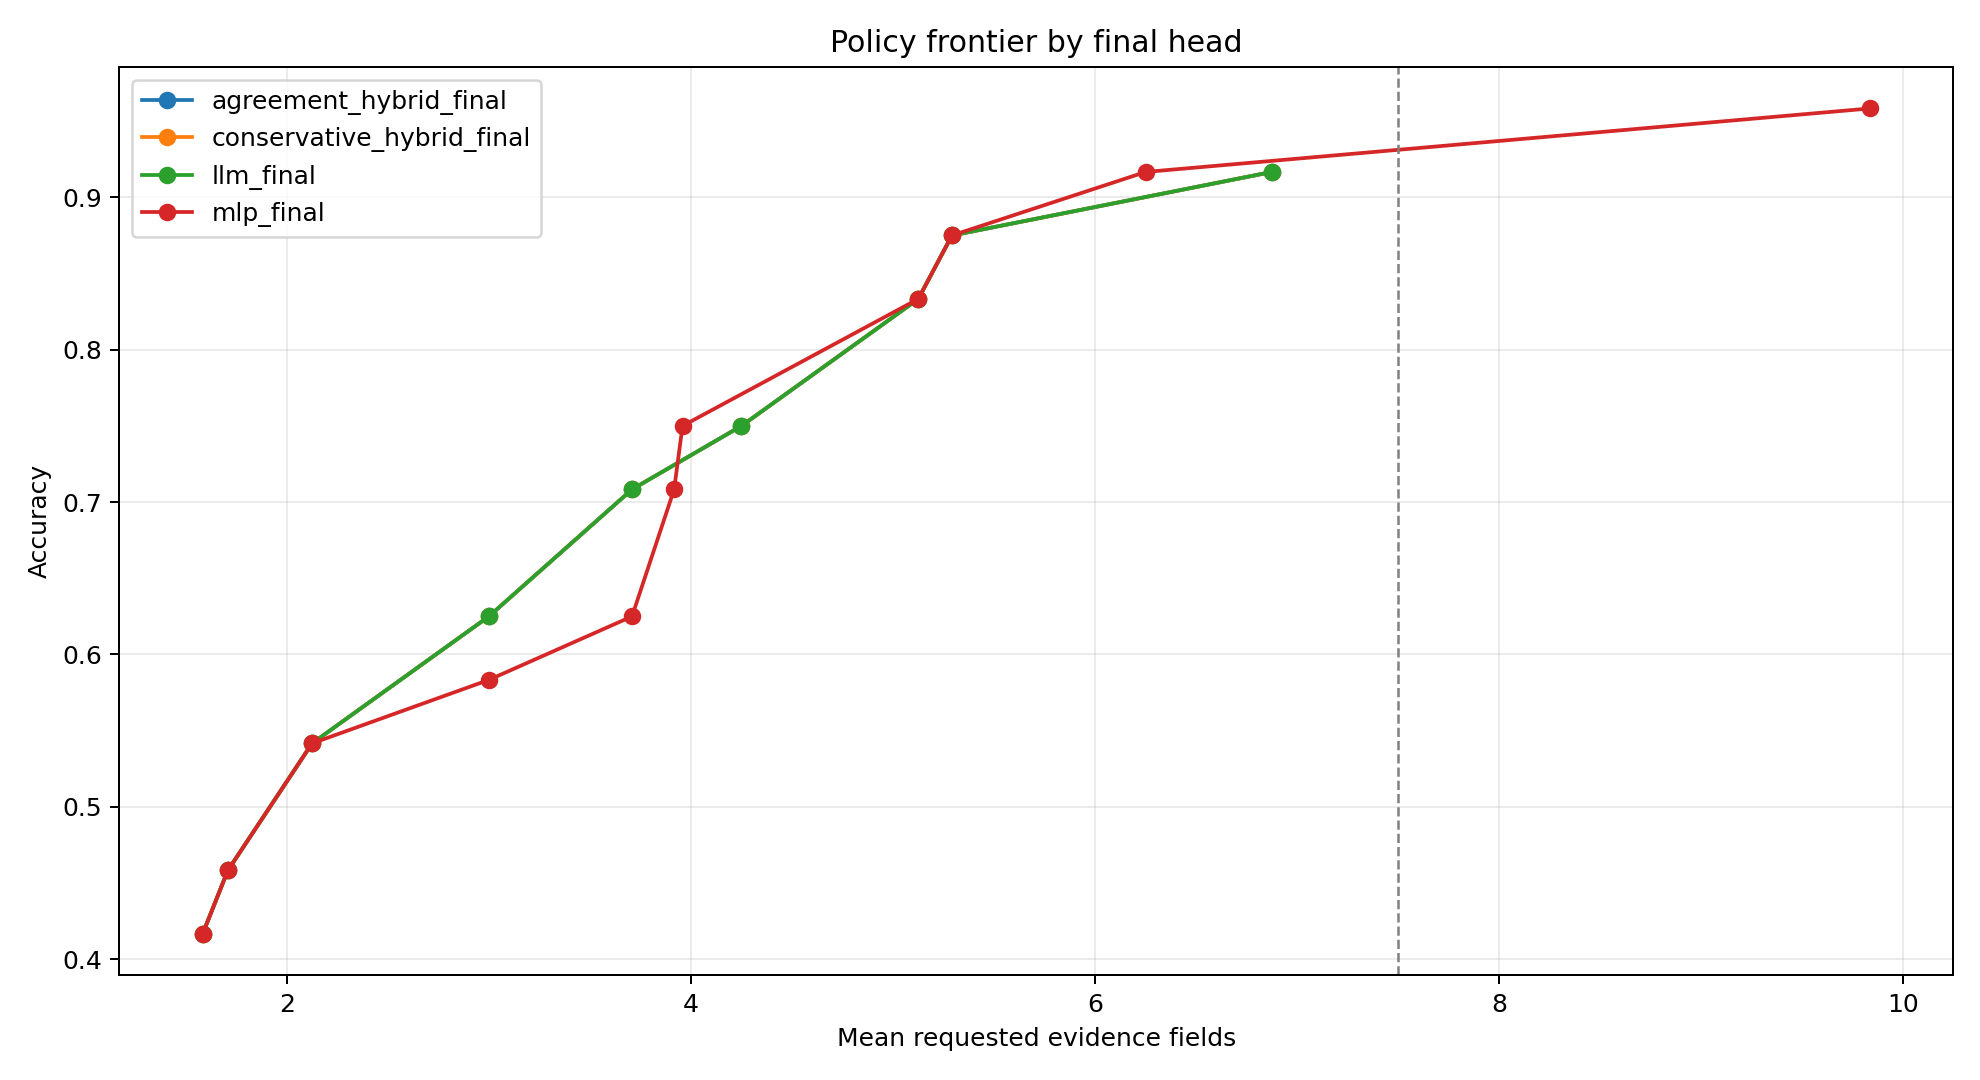
\includegraphics[width=0.82\linewidth]{artifacts/stopping_policy_ablation/stopping_policy_ablation_24case_v1/figures/policy_frontier_accuracy.png}
\caption{Offline stopping-policy frontier. The selected MLP-guided stop rule gives a better accuracy/request tradeoff than aggressive LLM-only stopping.}
\end{figure}

\section{Main Live Confirmation}

The frozen Notebook 13 49-case confirmation is the main defended live result.

\begin{table}[H]
\centering
\caption{Notebook 13 selected MLP-stop live confirmation.}
\begin{tabular}{lr}
\toprule
Metric & Value \\
\midrule
Cases & 49 \\
Accuracy & $43/49 = 0.878$ \\
Top-3 accuracy & 0.918 \\
Top-5 accuracy & 0.939 \\
Macro-F1 & 0.845 \\
Mean requests & 6.59 \\
Median requests & 5.00 \\
Mean visible roots including initial & 7.59 \\
Stop-before-cap rate & 0.980 \\
Cap hits & 1 \\
Selected MLP stop fired & $36/49 = 0.735$ \\
LLM/MLP top-1 agreement & $46/49 = 0.939$ \\
\bottomrule
\end{tabular}
\end{table}

\begin{figure}[H]
\centering
\begin{subfigure}{0.48\linewidth}
\centering
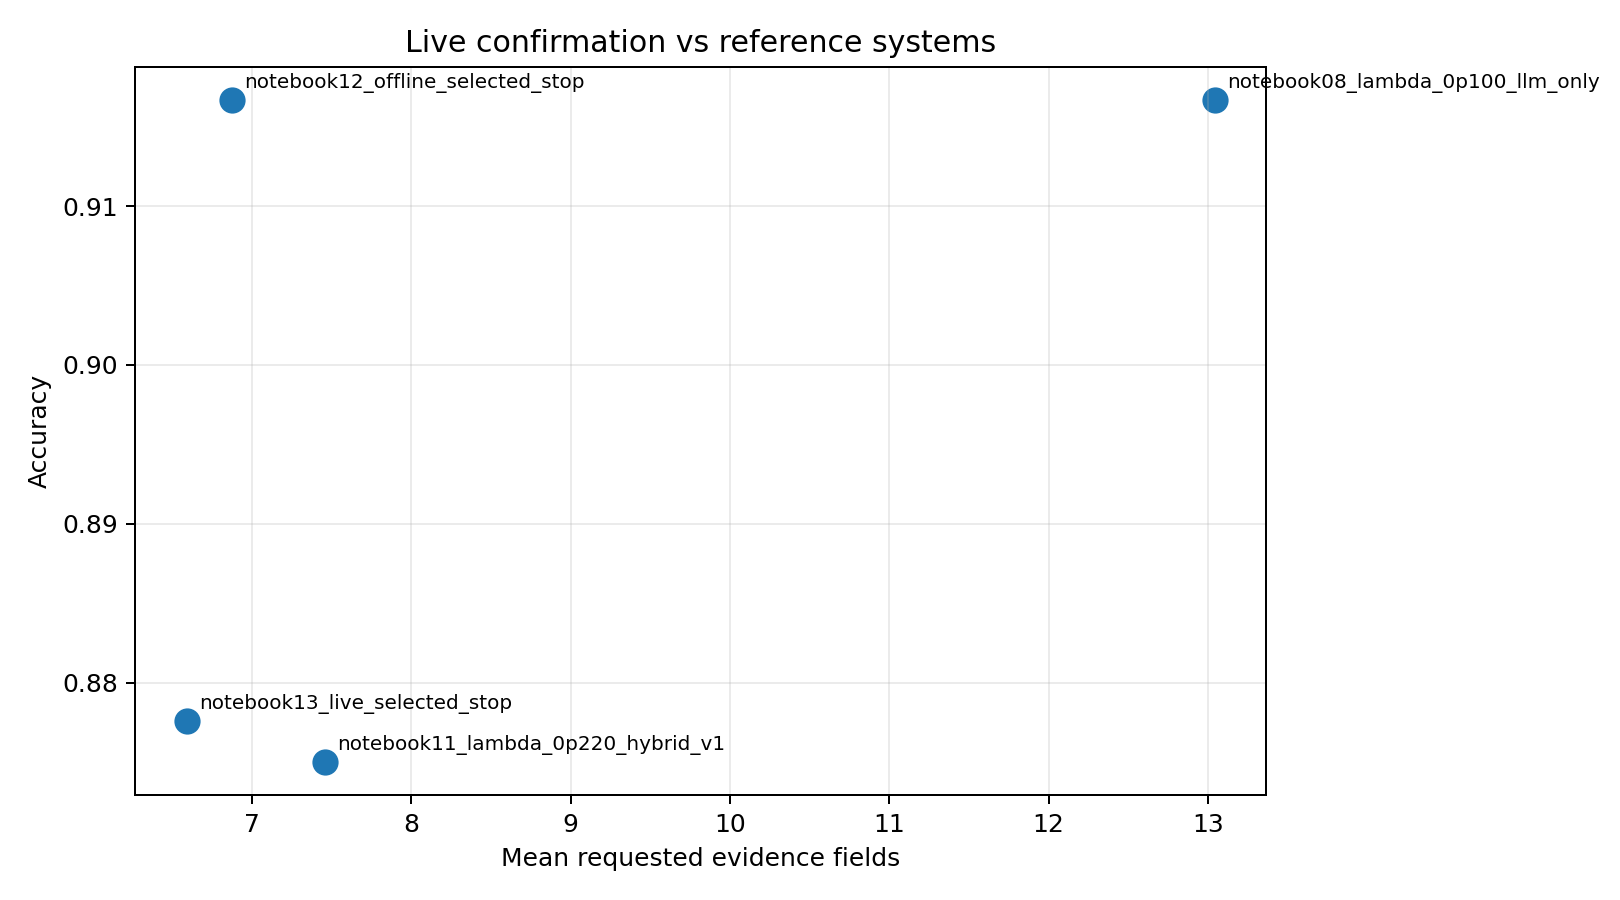
\includegraphics[width=\linewidth]{artifacts/sequential_hybrid_mlp_feedback/selected_stop_live_confirmation_49case_v1/figures/accuracy_vs_reference_requests.png}
\caption{Accuracy versus reference requests.}
\end{subfigure}
\hfill
\begin{subfigure}{0.48\linewidth}
\centering
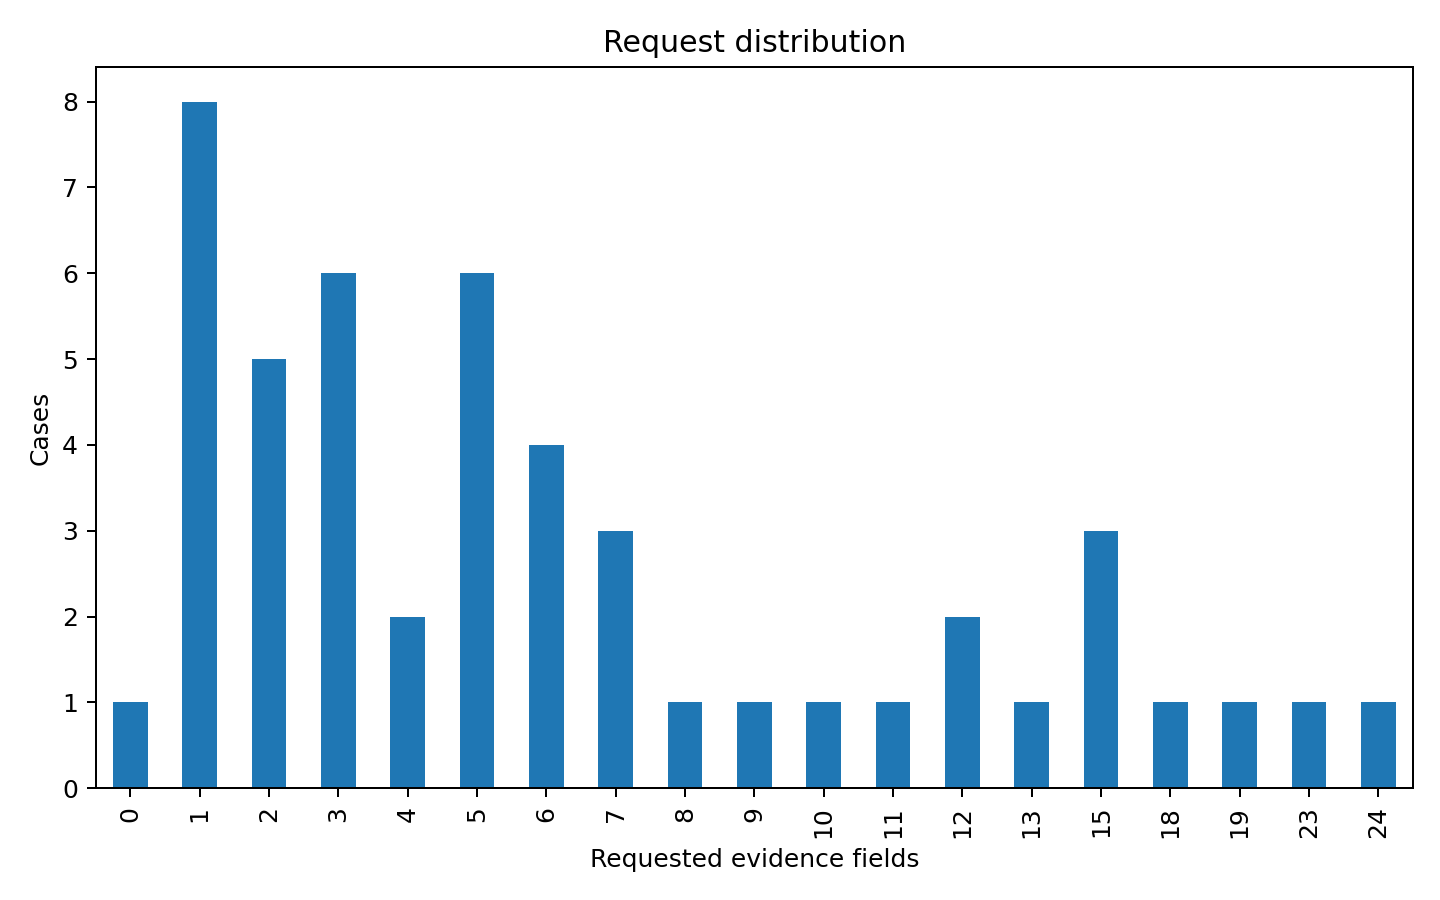
\includegraphics[width=\linewidth]{artifacts/sequential_hybrid_mlp_feedback/selected_stop_live_confirmation_49case_v1/figures/request_distribution.png}
\caption{Request distribution.}
\end{subfigure}
\caption{Notebook 13 final live confirmation figures.}
\end{figure}

\begin{figure}[H]
\centering
\begin{subfigure}{0.48\linewidth}
\centering
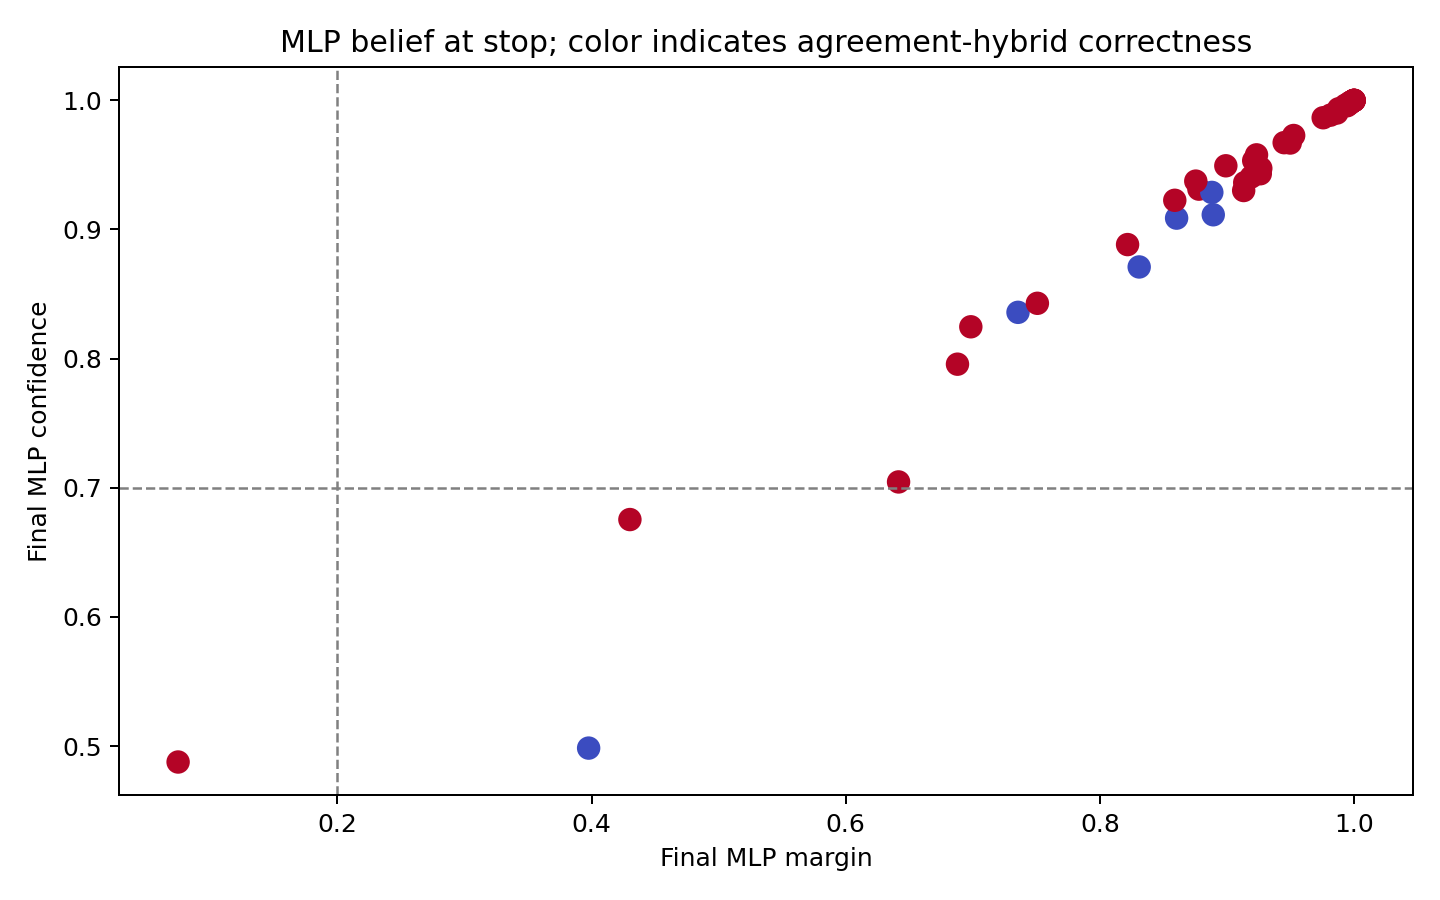
\includegraphics[width=\linewidth]{artifacts/sequential_hybrid_mlp_feedback/selected_stop_live_confirmation_49case_v1/figures/mlp_confidence_margin_at_stop.png}
\caption{MLP confidence and margin at stop.}
\end{subfigure}
\hfill
\begin{subfigure}{0.48\linewidth}
\centering
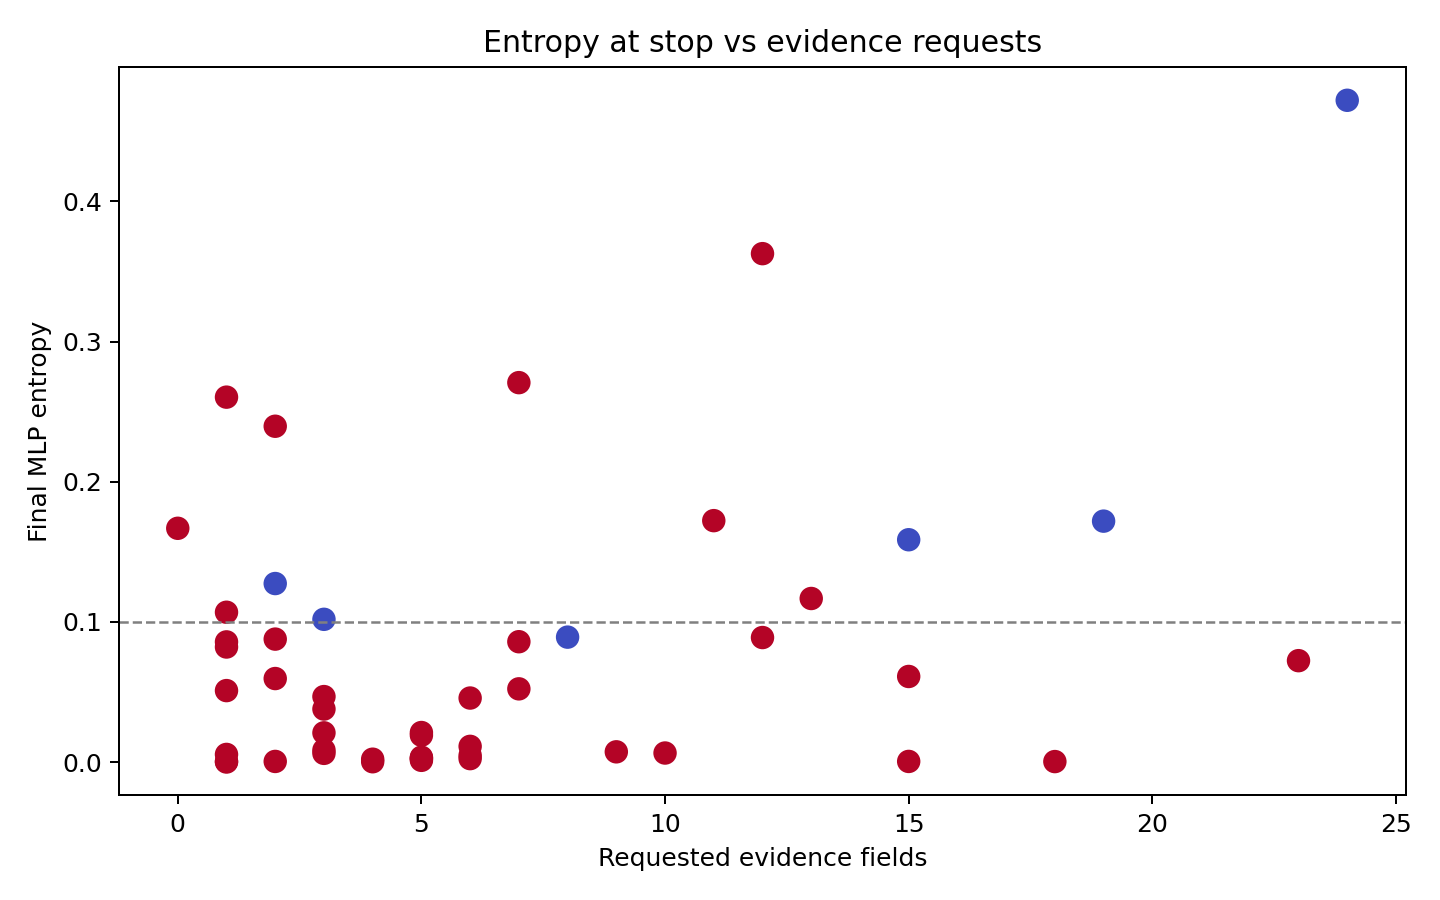
\includegraphics[width=\linewidth]{artifacts/sequential_hybrid_mlp_feedback/selected_stop_live_confirmation_49case_v1/figures/mlp_entropy_vs_requests.png}
\caption{MLP entropy versus request count.}
\end{subfigure}
\caption{The online MLP is used as a diagnostic belief monitor.}
\end{figure}

\section{Why the Design Decisions Were Made}

\subsection{Why Use an LLM for Evidence Acquisition?}

The \llm{} is strong at interpreting the current ledger, maintaining a differential, and choosing clinically plausible next questions. Early sequential results showed that \llm{} workup can recover a large fraction of the full-evidence gain. However, pure \llm{} stopping used many requests or became brittle at high evidence costs. The \llm{} was therefore retained as the controller but not trusted as the only stopping authority.

\subsection{Why Use an MLP for Stopping?}

The \mlp{} has two advantages. First, it is trained directly on \ddx{} structured evidence and produces calibrated-ish distributional signals over the 49 labels. Second, its confidence, margin, and entropy can be computed deterministically at every turn. The strongest empirical justification is Notebook 12: at similar request budget, the selected MLP-guided stop rule reaches $22/24$ while the best pure LLM stop reaches $20/24$.

\subsection{Why Not Let the MLP Choose Questions?}

Notebook 14 tested a direct MLP-discriminative shortlist using competing diagnoses and counterfactual entropy reduction. It fixed one hard case but introduced new errors and used more evidence.

\begin{table}[H]
\centering
\caption{Hybrid v2 question-shortlist ablation.}
\begin{tabular}{lrrr}
\toprule
System & Accuracy & Top-5 & Mean requests \\
\midrule
Hybrid v1 selected stop & 0.917 & 0.917 & 6.58 \\
Hybrid v2 MLP shortlist & 0.875 & 0.958 & 7.38 \\
\bottomrule
\end{tabular}
\end{table}

This led to an important design conclusion: the \mlp{} is useful as a belief and stop monitor, but direct MLP-driven question control is not automatically better.

\begin{figure}[H]
\centering
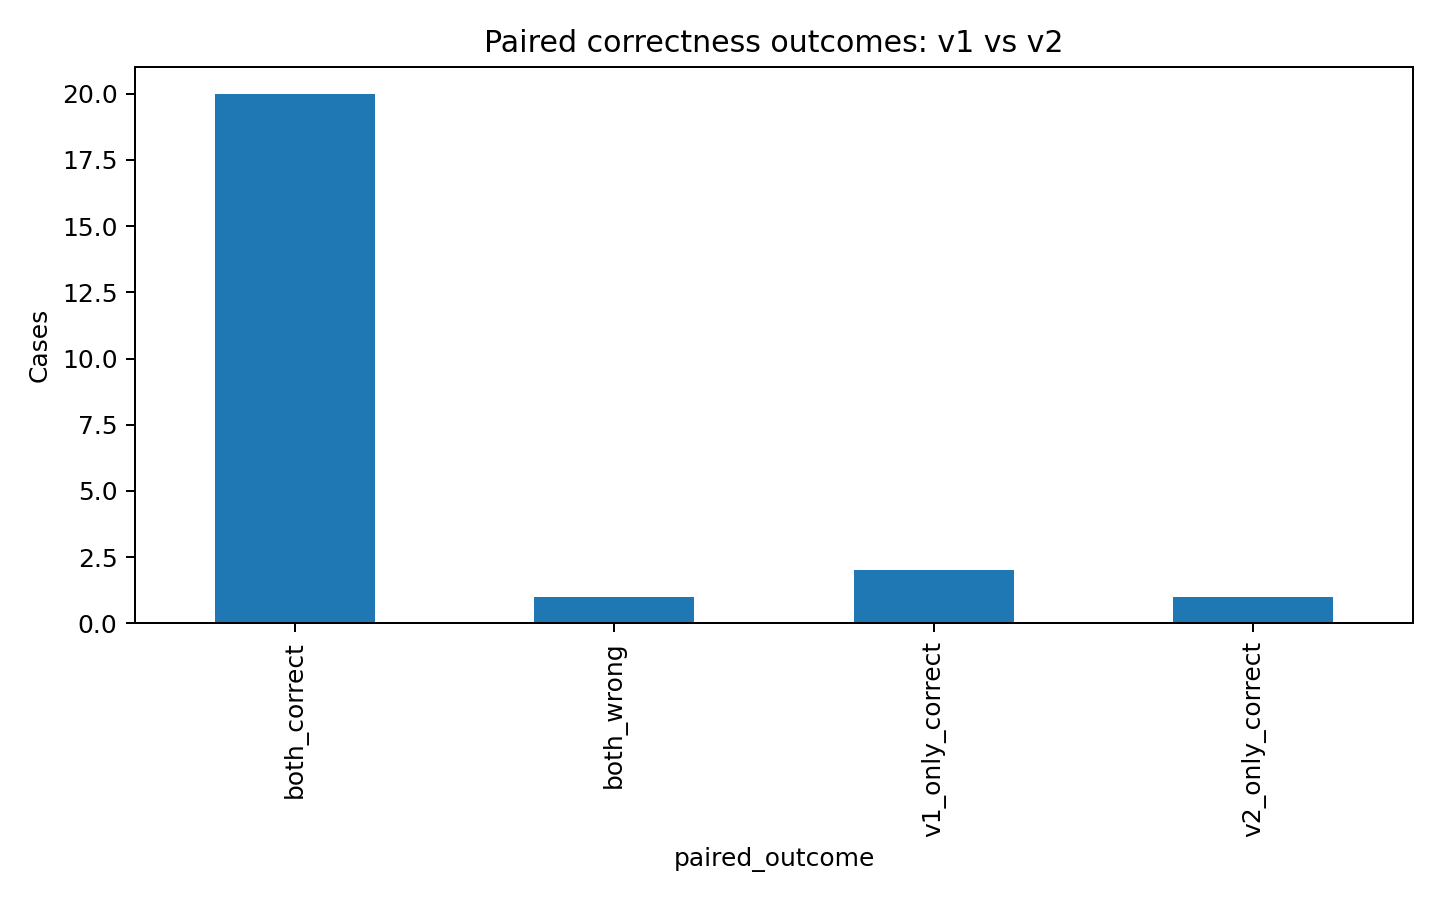
\includegraphics[width=0.75\linewidth]{artifacts/sequential_hybrid_mlp_feedback/hybrid_v2_mlp_discriminative_shortlist_24case_v1/figures/paired_correctness_outcomes.png}
\caption{Hybrid v2 paired correctness outcomes. The MLP shortlist introduced regressions, so it was rejected.}
\end{figure}

\section{Improvements and Novelty}

The project should not claim novelty as ``we used an LLM for diagnosis'' or ``we used a graph for medicine.'' Prior systems already study interactive diagnosis, medical agents, and graph-grounded reasoning. The real novelty is more specific: we built a \ddx{}-native, evidence-disciplined workup system that combines deterministic evidence control, neural belief feedback, matched-evidence evaluation, and graph/Bayesian critique.

\subsection{Improvement 1: From Static Classification to Evidence-Efficient Workup}

The first improvement is the move from one-shot classification to controlled evidence acquisition. The initial-evidence MLP establishes that the starting state is hard: $0.378$ full-test accuracy. The full-evidence MLP establishes that the dataset is highly diagnosable when evidence is available: $0.996$ accuracy. The proposed method targets the gap between those two settings. It asks a small number of fields and recovers much of the full-evidence benefit.

This is important because it changes the question from:
\[
\text{Can we classify a complete patient record?}
\]
to:
\[
\text{Which evidence should be acquired before diagnosis?}
\]
That is closer to real diagnostic workup and to the active feature acquisition literature.

\subsection{Improvement 2: Deterministic Evidence Ledger}

The evidence ledger is a major improvement over raw prompt history. It gives the system a structured source of truth:
\begin{itemize}[leftmargin=*]
    \item only initial evidence is visible at the start;
    \item hidden evidence is revealed only after a legal request;
    \item parent-child evidence gating prevents invalid questions;
    \item every reveal is decoded into human-readable clinical language;
    \item every request and diagnosis state is auditable after the run.
\end{itemize}

This improves both scientific fairness and interpretability. The \llm{} cannot silently inspect the whole case, and the evaluator can reconstruct exactly what was known at each turn.

\subsection{Improvement 3: Separating Evidence Acquisition from Stopping}

The final promoted architecture separates two roles:
\[
\text{\llm{} chooses evidence} \qquad \text{and} \qquad \text{\mlp{} decides whether enough evidence is visible.}
\]
This is the main practical improvement. The \llm{} remains useful for selecting clinically plausible next questions, but it is not trusted as the only confidence source. The partial-evidence \mlp{} supplies confidence, margin, entropy, stability, and agreement signals after every update.

The ablation supports this design. At similar request budgets, the selected MLP-guided stop rule reaches $0.917$ accuracy on the 24-case control, while the best pure LLM stop reaches $0.833$. The final 49-case Notebook 13 run reaches $0.878$ accuracy with only $6.59$ mean requests, and a fresh Notebook 13-style live run reaches $0.918$ with $6.20$ requests.

\subsection{Improvement 4: Matched-Evidence Evaluation}

A common weakness in sequential-agent projects is that they report only the final agent answer. We added matched-evidence evaluation to ask a stricter question: if a neural classifier receives the same evidence acquired by the agent, how well does it perform?

This matters because it separates:
\[
\text{value from acquiring good evidence}
\]
from:
\[
\text{value from the final reasoner using that evidence.}
\]
The partial-evidence MLP showed that the acquired evidence itself is valuable and that the final LLM answer is not always the only useful head. This directly motivated the hybrid architecture.

\subsection{Improvement 5: Negative Ablations as Design Evidence}

Several attempted improvements were rejected:
\begin{itemize}[leftmargin=*]
    \item direct MLP-guided question shortlisting;
    \item hard MedKGI-style graph top-10 shortlisting;
    \item graph-advisory shortlist blending;
    \item offline Bayesian VOI as a full replacement controller;
    \item live graph/Bayes rescue as a promoted improvement;
    \item live targeted branching as a final promoted multi-agent method.
\end{itemize}

These negative results are part of the contribution. They show that the final architecture was not chosen by intuition alone. The project tested plausible research directions and kept the one that survived live confirmation: LLM-led acquisition plus MLP-guided stopping.

\subsection{Improvement 6: Graph/Bayesian Critique Without Overclaiming}

The graph and Bayesian work adds an algorithmic analysis layer. The train-derived graph posterior can detect support and contradiction in final evidence states. The conservative graph critic improves the saved Notebook 13 trace from $43/49$ to $44/49$ without new requests. The calibrated offline graph/Bayes rescue reaches $47/49$ with $6.96$ mean requests.

However, live confirmation did not promote the rescue layer. This is scientifically useful: it shows graph/Bayesian signals are promising as critics and rescue candidates, but they need stronger calibration before becoming the defended live method.

\subsection{Novelty Statement}

The most defensible novelty statement is:
\begin{quote}
This project contributes a \ddx{}-native evidence-efficient diagnostic workup pipeline that combines a deterministic evidence ledger, an \llm{} evidence-acquisition controller, a BASD-style partial-evidence \mlp{} stopping monitor, matched-evidence neural evaluation, and graph/Bayesian post-hoc critique. The main promoted improvement is not generic agentic diagnosis, but evidence-disciplined sequential workup with neural stop certification and extensive live/ablation evidence.
\end{quote}

\section{Graph-Ledger Experiments}

\subsection{MedKGI-Style Graph Analysis}

Notebook 16 builds train-derived disease/evidence graph statistics: information gain, disease-specific support, contradiction, graph rank, and terminal graph scores. Offline replay shows the graph contains signal. Incorrect Notebook 13 trajectories had worse mean graph rank and lower information gain than correct ones. This justified testing graph-guided live policies.

\begin{figure}[H]
\centering
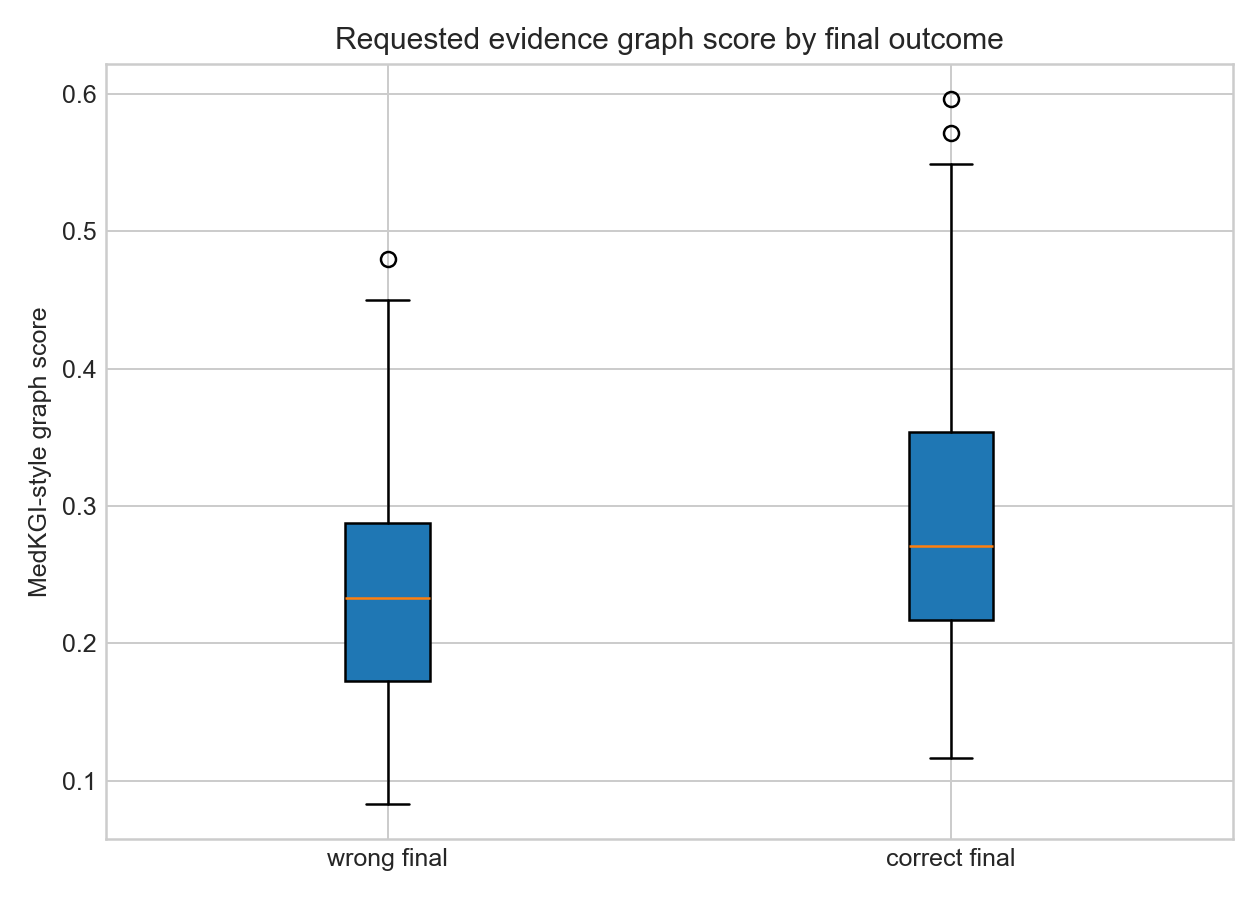
\includegraphics[width=0.76\linewidth]{artifacts/graph_algorithmic_ledger/medkgi_style_offline_notebook13_49case_v1/figures/request_score_correct_vs_wrong.png}
\caption{Graph request score differs between correct and wrong trajectories, indicating useful diagnostic signal.}
\end{figure}

\subsection{Hard Graph Shortlist and Advisory Graph Shortlist}

Notebook 17 replaces the broad Notebook 13 shortlist with a hard graph top-10 legal field list. It asks high-ranking graph questions but underperforms. Notebook 18 restores shortlist diversity and adds graph advisory scoring, but still fails to beat Notebook 13.

\begin{table}[H]
\centering
\caption{Graph shortlist ablations on 24 cases.}
\begin{tabular}{lrrr}
\toprule
System & Accuracy & Top-5 & Mean requests \\
\midrule
Hybrid v1 selected stop & 0.917 & 0.917 & 6.58 \\
Hard MedKGI graph shortlist & 0.833 & 0.875 & 6.21 \\
Graph-advisory hybrid shortlist & 0.875 & 0.917 & 7.67 \\
\bottomrule
\end{tabular}
\end{table}

The lesson is subtle: graph scores are locally meaningful but can over-constrain the action space. The graph may efficiently ask high-scoring questions for the wrong active differential.

\section{Bayesian Value-of-Information Ledger}

Notebook 19 implements an offline Bayesian value-of-information controller. It builds train-only likelihood tables:
\[
P(D),\quad P(\text{age bin}\mid D),\quad P(\text{sex}\mid D),\quad P(\text{root outcome}\mid D),
\]
then fuses Bayesian and \mlp{} posteriors by log-linear pooling:
\[
p_{\text{fused}} = \operatorname{softmax}\left(0.60\log p_{\mlp} + 0.40\log p_{\text{Bayes}}\right).
\]
Candidate evidence roots are scored by:
\[
\begin{aligned}
U(a) ={}& 0.55\,\Delta H_{\text{fused}}(a)
 + 0.20\,\Delta \text{margin}(a)\\
&+0.15\,\text{contradiction\_resolution}(a)
 +0.10\,\text{rare\_recovery}(a)
 - \lambda - \text{redundancy}.
\end{aligned}
\]

Despite the mathematical appeal, the full 49-case result is negative.

\begin{table}[H]
\centering
\caption{Notebook 19 Bayesian VOI policy sweep.}
\begin{tabular}{rrrrrr}
\toprule
$\lambda$ & Correct & Accuracy & Top-5 & Macro-F1 & Mean requests \\
\midrule
0.00 & 33/49 & 0.673 & 0.878 & 0.620 & 22.37 \\
0.02 & 26/49 & 0.531 & 0.837 & 0.461 & 7.98 \\
0.05 & 26/49 & 0.531 & 0.776 & 0.447 & 5.65 \\
0.10 & 25/49 & 0.510 & 0.776 & 0.424 & 4.43 \\
0.15 & 24/49 & 0.490 & 0.776 & 0.396 & 4.33 \\
\bottomrule
\end{tabular}
\end{table}

The failure diagnosis is important. The VOI controller over-selects globally informative generic fields, creates evidence trajectories unlike the policy-shaped masks used to train the partial-evidence \mlp{}, and becomes confidently wrong. This is a negative result, but it clarifies that posterior control must be trajectory-aware and clinically targeted.

\begin{figure}[H]
\centering
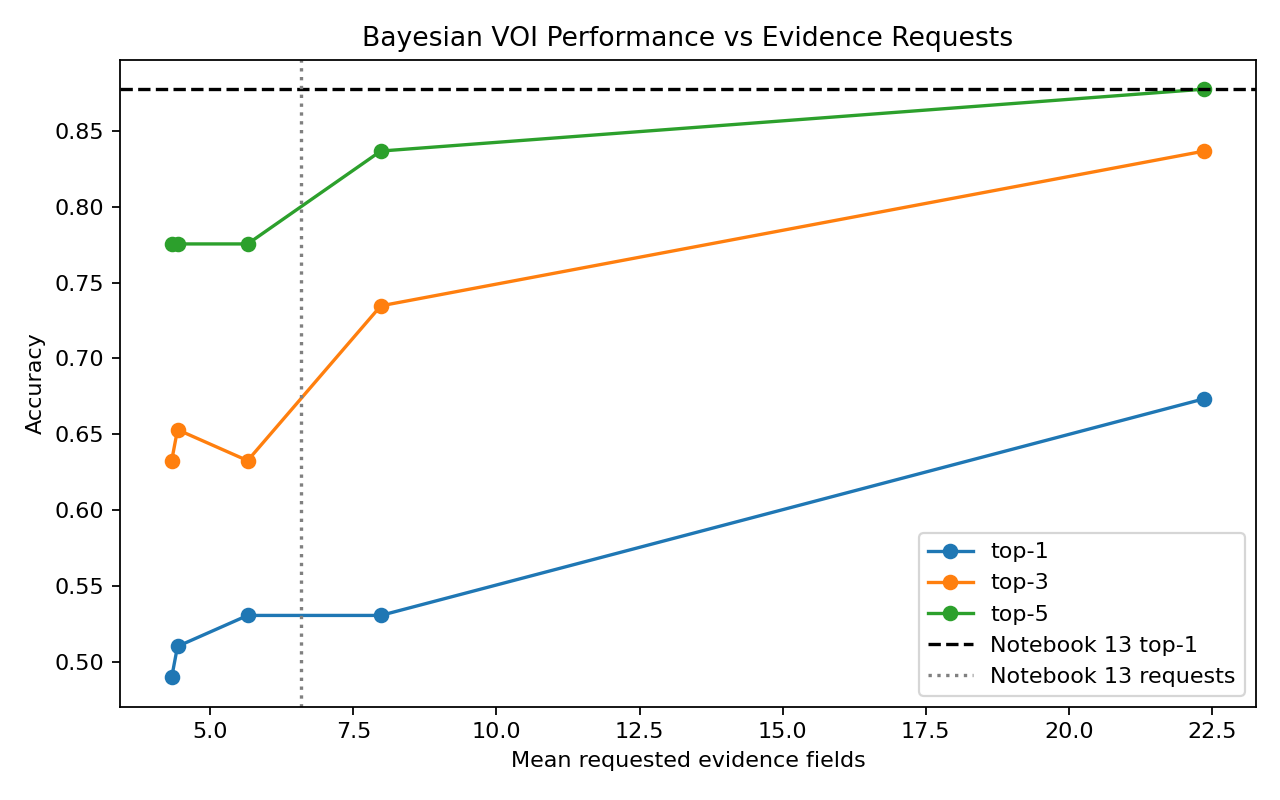
\includegraphics[width=0.80\linewidth]{artifacts/bayesian_voi_ledger/bayesian_voi_offline_notebook13_49case_v1/figures/accuracy_topk_vs_mean_requests.png}
\caption{Bayesian VOI did not dominate the Notebook 13 hybrid frontier.}
\end{figure}

\section{Graph Posterior Critic and Calibrated Rescue}

\subsection{Graph Posterior Final Critic}

Notebook 22 keeps Notebook 13 evidence acquisition fixed and applies a conservative graph posterior critic at the final state. The graph score is a clipped signed log-odds support sum:
\[
\text{graph\_score}(d)=\sum_{e \in O_T}\operatorname{clip}(\log \operatorname{odds}(e \rightarrow d),-3,3).
\]
The critic overrides only when the graph top-1 differs, has sufficient margin, the original prediction has negative support, and the graph candidate has positive support.

\begin{table}[H]
\centering
\caption{Graph posterior final critic.}
\begin{tabular}{lrrrrr}
\toprule
System & Cases & Accuracy & Top-3 & Top-5 & Mean requests \\
\midrule
Notebook 13 selected stop & 49 & 0.878 & 0.918 & 0.939 & 6.59 \\
Notebook 22 graph critic & 49 & 0.898 & 0.939 & 0.939 & 6.59 \\
\bottomrule
\end{tabular}
\end{table}

The critic fires once and fixes Croup without regressions. It is a useful offline final-head enhancement but not a live-confirmed policy.

\subsection{Calibrated Graph/Bayes Rescue}

Notebook 23 extends this into a calibrated offline rescue reranker. It uses train/validate-derived synthetic partial states, graph support, Bayesian posterior features, \mlp{} features, prior recovery, and up to three rescue questions for suspicious early stops.

\begin{table}[H]
\centering
\caption{Offline calibrated graph/Bayes rescue.}
\begin{tabular}{lrrrr}
\toprule
System & Cases & Accuracy & Mean requests & Regressions \\
\midrule
Notebook 13 selected stop & 49 & 0.878 & 6.59 & 0 \\
Notebook 22 graph critic & 49 & 0.898 & 6.59 & 0 \\
Notebook 23 graph/Bayes rescue & 49 & 0.959 & 6.96 & 0 \\
\bottomrule
\end{tabular}
\end{table}

It fixes four saved-trace misses: COPD, Croup, Influenza, and Unstable angina. However, Notebook 24 tests the frozen rescue inside a fresh live run, and it does not reproduce the offline gain.

\begin{table}[H]
\centering
\caption{Live rescue confirmation. The base reproduced strongly; the rescue layer was not promoted.}
\begin{tabular}{lrrrrr}
\toprule
System & Cases & Accuracy & Top-3 & Top-5 & Mean requests \\
\midrule
Original Notebook 13 artifact & 49 & 0.878 & 0.918 & 0.939 & 6.59 \\
Notebook 23 offline rescue & 49 & 0.959 & -- & -- & 6.96 \\
Notebook 24 fresh live base & 49 & 0.918 & 0.939 & 0.939 & 6.20 \\
Notebook 24 live rescue & 49 & 0.918 & 0.939 & 0.939 & 6.39 \\
\bottomrule
\end{tabular}
\end{table}

\begin{figure}[H]
\centering
\begin{subfigure}{0.48\linewidth}
\centering
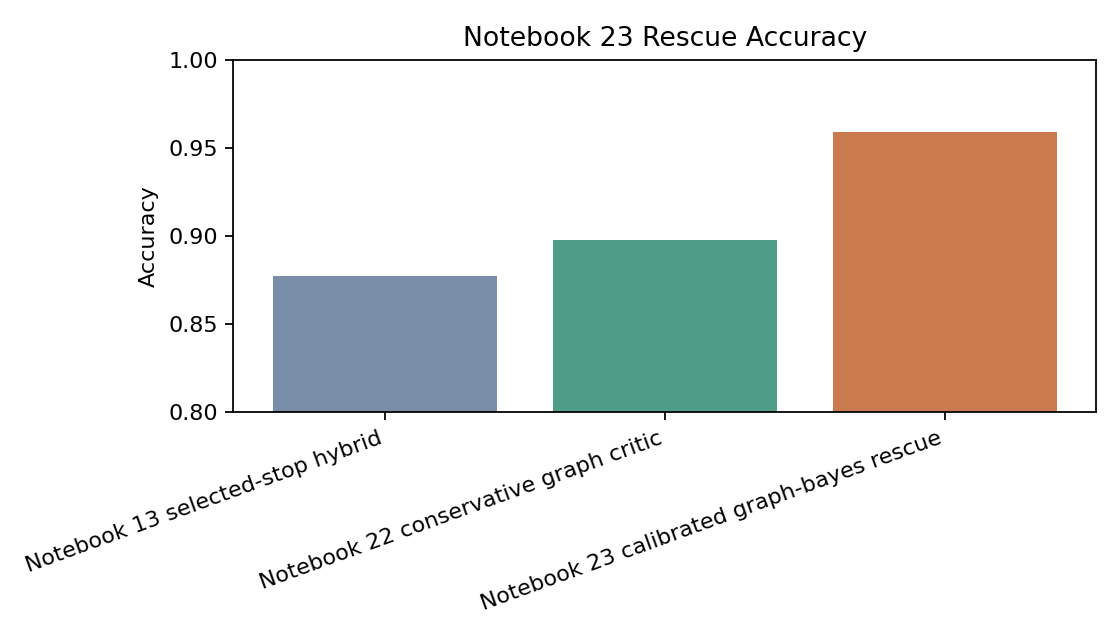
\includegraphics[width=\linewidth]{artifacts/graph_algorithmic_ledger/calibrated_graph_bayes_rescue_reranker_49case_v1/figures/accuracy_comparison.png}
\caption{Offline rescue comparison.}
\end{subfigure}
\hfill
\begin{subfigure}{0.48\linewidth}
\centering
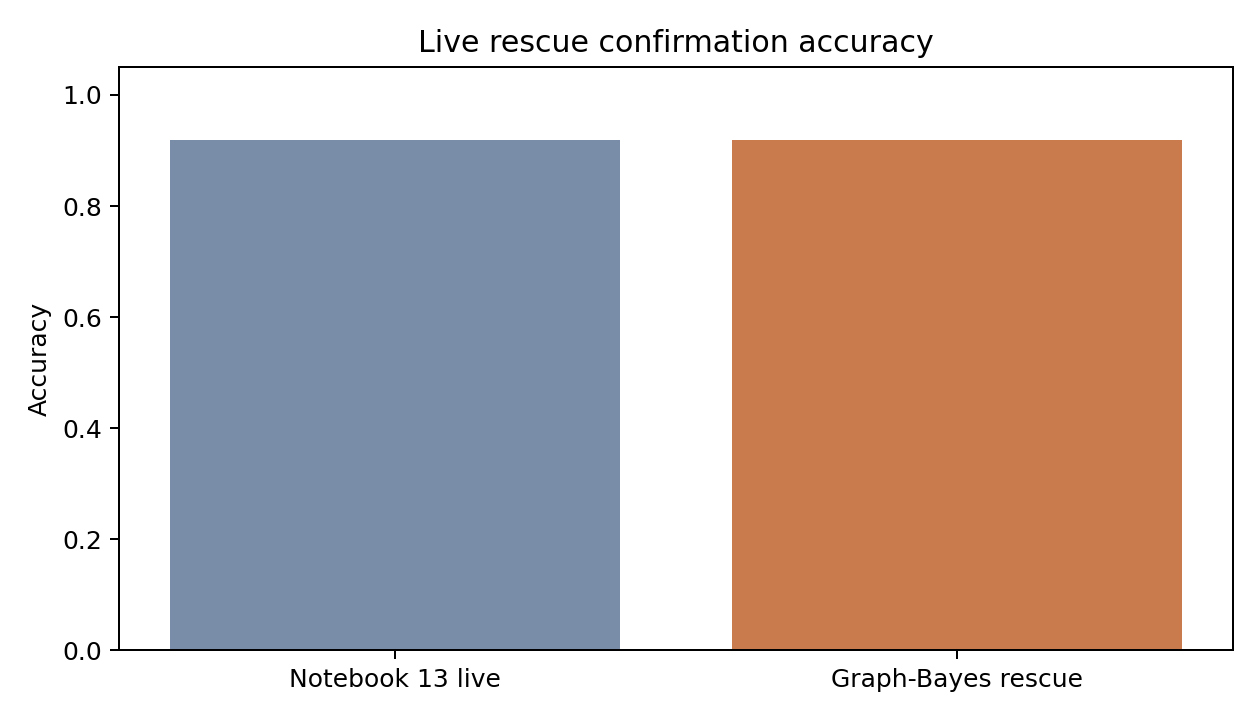
\includegraphics[width=\linewidth]{artifacts/graph_algorithmic_ledger/live_graph_bayes_rescue_confirmation_49case_v1/figures/accuracy_comparison.png}
\caption{Live rescue confirmation.}
\end{subfigure}
\caption{The offline rescue was strong but did not promote under fresh live confirmation.}
\end{figure}

\section{Trajectory Replicates and Targeted Branching}

Notebook 25 collects three additional Notebook 13-style base trajectories. Notebook 26 analyzes five total trajectories: original Notebook 13, Notebook 24 base, and three Notebook 25 replicates.

\begin{table}[H]
\centering
\caption{Observed base trajectory variability.}
\begin{tabular}{lrr}
\toprule
Run & Accuracy & Mean requests \\
\midrule
Notebook 13 frozen & 43/49 = 0.878 & 6.59 \\
Notebook 24 base & 45/49 = 0.918 & 6.20 \\
Notebook 25 r01 & 44/49 = 0.898 & 7.00 \\
Notebook 25 r02 & 42/49 = 0.857 & 7.02 \\
Notebook 25 r03 & 42/49 = 0.857 & 6.82 \\
\bottomrule
\end{tabular}
\end{table}

Across five trajectories, majority vote stays at $43/49$, while oracle best-of-five reaches $47/49$. This means the opportunity is not naive voting; it is selective branching and adjudication.

Notebook 26 also tests diagnostic branch policies offline over the observed trajectories. The strongest Notebook 13-base diagnostic policy uses a sparse suspicion trigger, at most two alternate branches, and a Bayesian posterior judge. It reaches $47/49$ with zero regressions in replay, a branch trigger rate of $0.184$, mean selected requests $6.86$, and mean total branch requests $9.18$. This result is not promoted because it reuses observed trajectories, but it provides the clearest algorithmic reason to try prospective branching: some wrong trajectories are recoverable if the system branches only at suspicious states and adjudicates with graph/Bayes/MLP signals.

\begin{figure}[H]
\centering
\begin{subfigure}{0.48\linewidth}
\centering
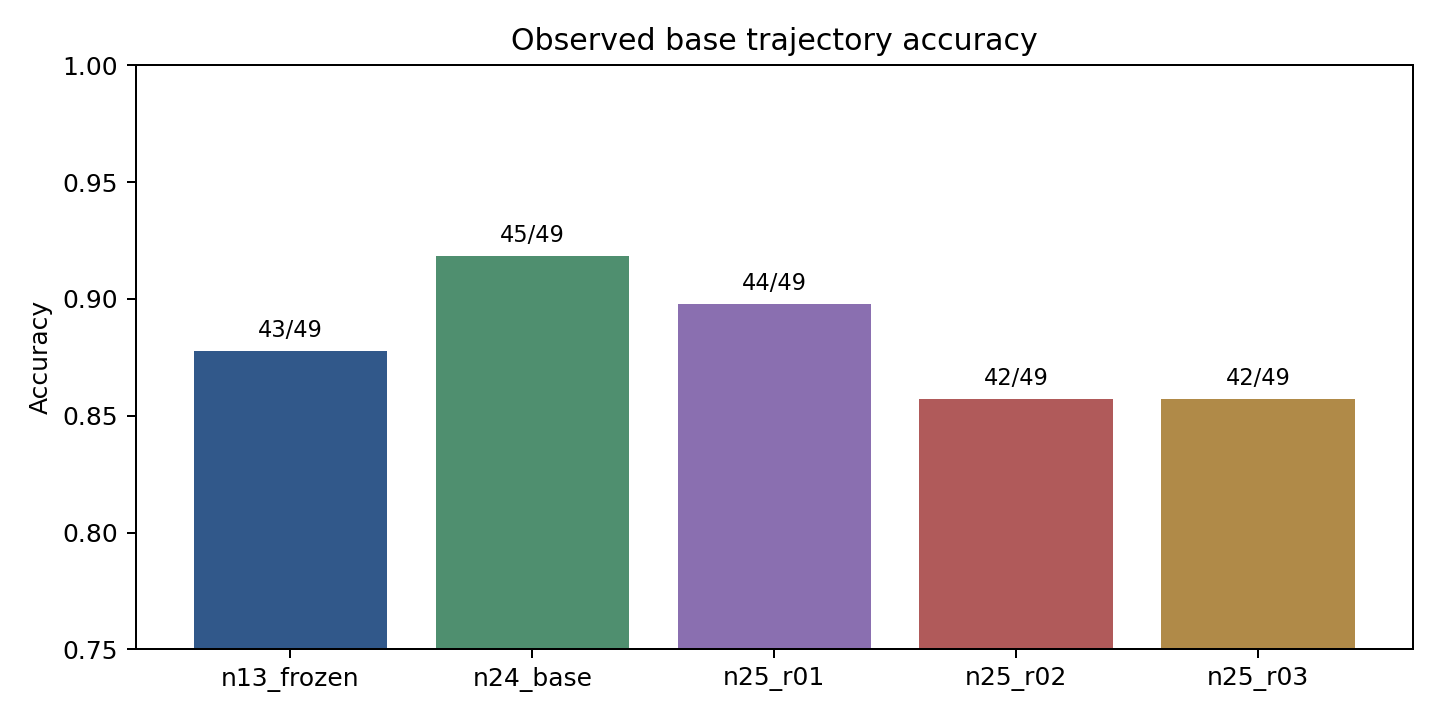
\includegraphics[width=\linewidth]{artifacts/trajectory_replicates/offline_branching_trajectory_lab_49case_v1/figures/observed_run_accuracy.png}
\caption{Accuracy of observed base trajectories.}
\end{subfigure}
\hfill
\begin{subfigure}{0.48\linewidth}
\centering
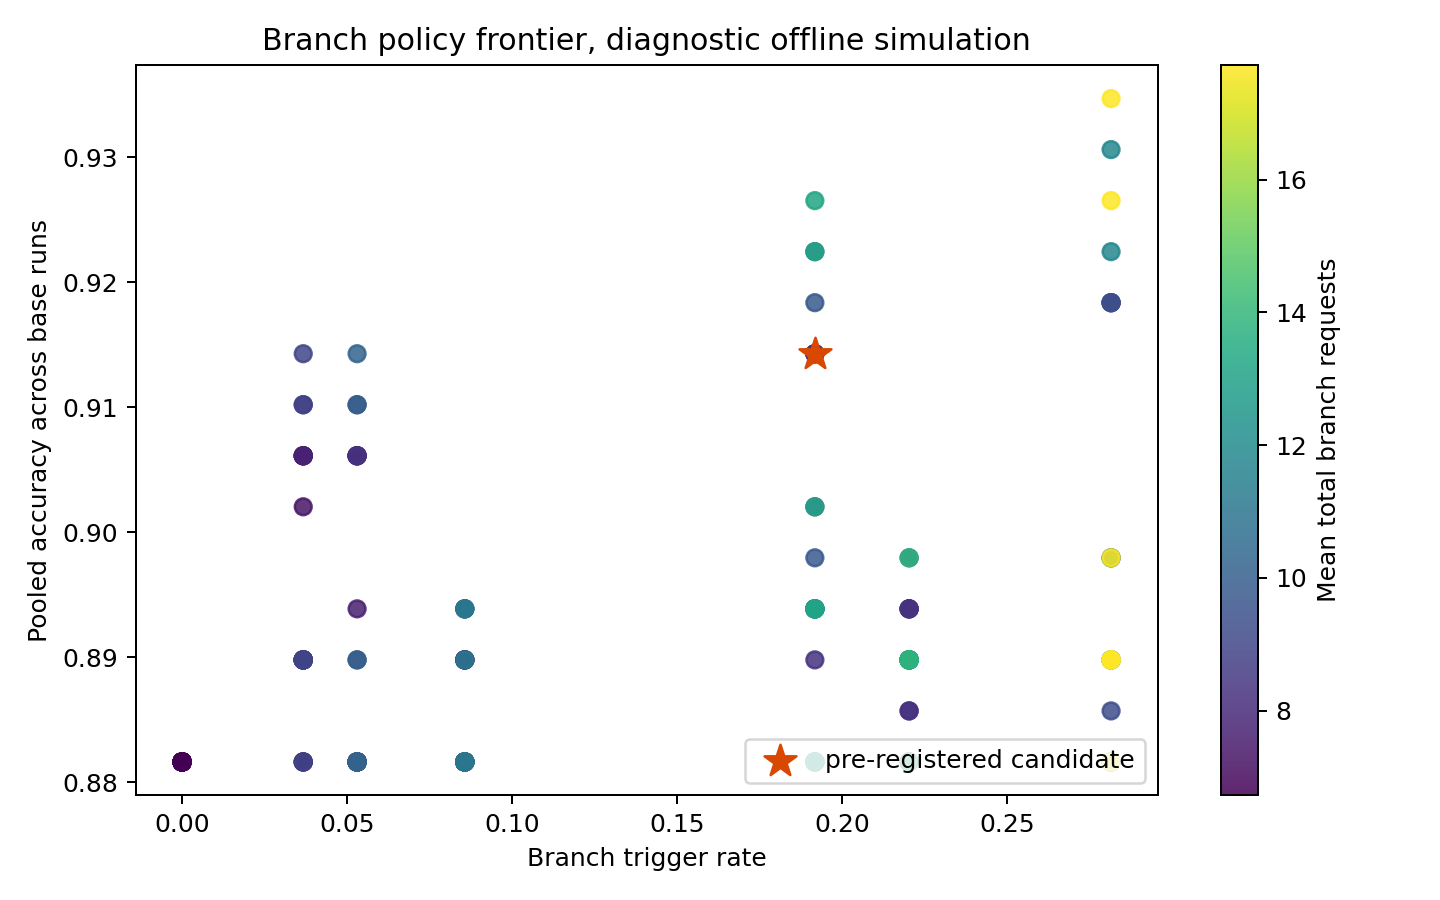
\includegraphics[width=\linewidth]{artifacts/trajectory_replicates/offline_branching_trajectory_lab_49case_v1/figures/branch_policy_frontier.png}
\caption{Offline branch policy frontier.}
\end{subfigure}
\caption{Notebook 26 shows that trajectory diversity has value, but only with selective branching and a resolver.}
\end{figure}

Notebook 27 implements a prospective targeted branching confirmation. It runs one base workup, triggers at most two fresh-context branches only when suspicious, and adjudicates with a raw Bayesian posterior plus graph/\mlp{} tie signals.

\begin{table}[H]
\centering
\caption{Live targeted branching confirmation.}
\begin{tabular}{lr}
\toprule
Metric & Value \\
\midrule
Base accuracy & $42/49 = 0.857$ \\
Targeted branching accuracy & $43/49 = 0.878$ \\
Wins vs base & 2 \\
Regressions vs base & 1 \\
Branch trigger rate & 0.184 \\
Mean selected requests & 6.82 \\
Mean total branch requests & 11.45 \\
Promotion decision & Not promoted \\
\bottomrule
\end{tabular}
\end{table}

\begin{figure}[H]
\centering
\begin{subfigure}{0.48\linewidth}
\centering
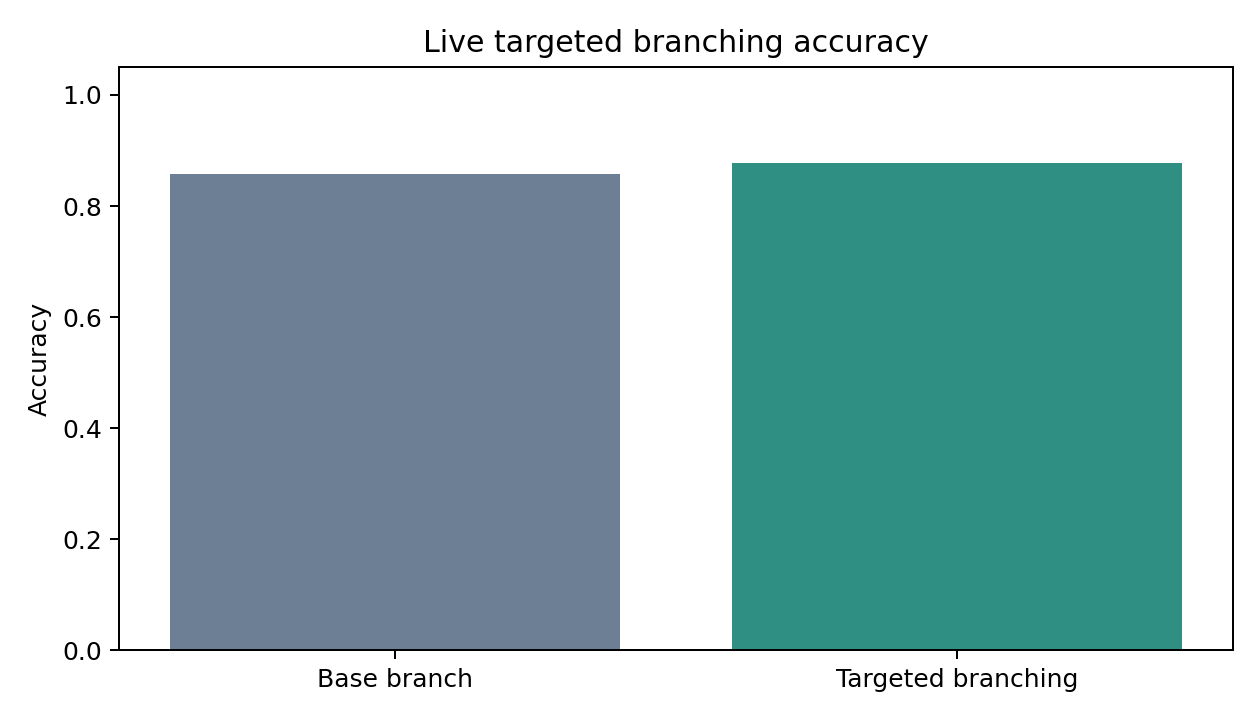
\includegraphics[width=\linewidth]{artifacts/trajectory_replicates/live_targeted_branching_confirmation_49case_v1/figures/accuracy_comparison.png}
\caption{Accuracy comparison.}
\end{subfigure}
\hfill
\begin{subfigure}{0.48\linewidth}
\centering
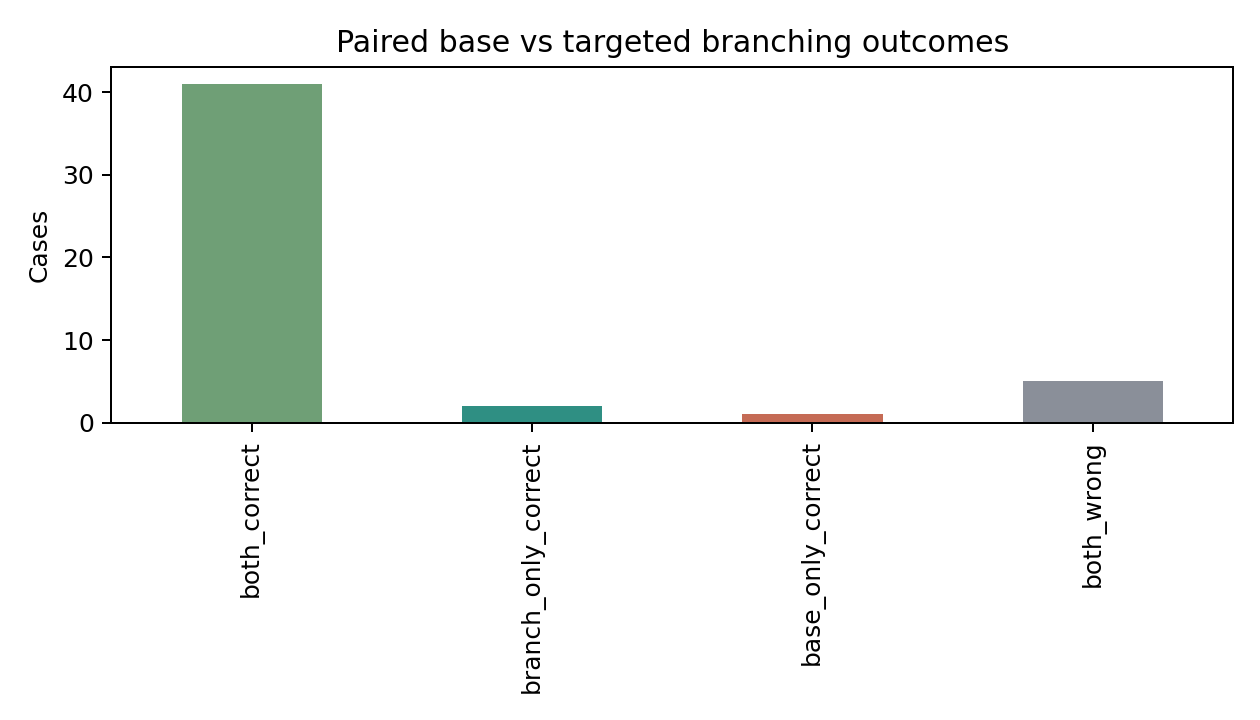
\includegraphics[width=\linewidth]{artifacts/trajectory_replicates/live_targeted_branching_confirmation_49case_v1/figures/paired_outcomes.png}
\caption{Paired outcomes.}
\end{subfigure}
\caption{Targeted branching recovered some wrong trajectories but introduced a regression and increased total request cost.}
\end{figure}

\subsection{Notebook 28: MLP-Gated Confounder Graph/Bayes Branching}

Notebook 28 is the successor to Notebook 27. It keeps the Notebook 13-style base workup, but changes the branching layer in three ways:
\begin{itemize}[leftmargin=*]
    \item it replaces the hand-written \texttt{hybrid\_suspicion\_v1} trigger with a learned branch-trigger MLP trained on train/validate synthetic partial evidence states;
    \item it adds confounder-pair coverage features so the branch gate can detect unresolved disease neighborhoods, not only low confidence or direct contradiction;
    \item it expands the resolver candidate pool to include real branch outputs plus graph, Bayes, and MLP pseudo-candidates, with base protection when the base answer is graph rank 1 and Bayes rank 1.
\end{itemize}

The branch-trigger MLP is trained to estimate whether the current base terminal state is likely to be a wrong anchor. Its selected threshold is $0.375$. On validation states, the branch gate reaches AUC $0.954$, average precision $0.931$, precision $0.823$, recall $0.940$, and branch rate $0.499$ at the selected threshold. The candidate resolver is also trained on synthetic train/validate candidate rows and reaches AUC $0.955$ and average precision $0.809$.

Conceptually, Notebook 28 changes the branching policy from:
\[
\text{hand-written suspicion signals} \rightarrow \text{fresh branches} \rightarrow \text{raw Bayes judge}
\]
to:
\[
\text{learned branch gate} \rightarrow \text{fresh branches + pseudo-candidates} \rightarrow \text{calibrated graph/Bayes/MLP resolver}.
\]

\begin{table}[H]
\centering
\caption{Notebook 28 live MLP-gated confounder branching result.}
\begin{tabular}{lr}
\toprule
Metric & Value \\
\midrule
Cases & 49 \\
Same-run base accuracy & $42/49 = 0.857$ \\
Notebook 28 selected accuracy & $44/49 = 0.898$ \\
Top-3 / Top-5 accuracy & 0.959 / 0.959 \\
Macro-F1 & 0.864 \\
Wins vs base & 2 \\
Regressions vs base & 0 \\
Changed predictions & 2 \\
Branch trigger rate & 0.082 \\
Branches spawned & 12 \\
Mean selected requests & 6.63 \\
Mean base requests & 6.92 \\
Mean total branch requests & 9.96 \\
Promotion decision & Not promoted \\
\bottomrule
\end{tabular}
\end{table}

Notebook 28 is better than Notebook 27 on the main branching safety issue: it improves its same-run base by two cases with zero regressions, whereas Notebook 27 had two wins and one regression. Its selected predictions come mostly from the base branch, with one \texttt{counteranchor\_scout} selection and one \texttt{pseudo\_graph\_top1} selection. However, it still reaches only $44/49$, below the $47/49$ target suggested by offline branching and below the strongest fresh Notebook 13-style base run. Therefore it is best reported as a positive branching-safety improvement, not as the defended final method.

\begin{figure}[H]
\centering
\begin{subfigure}{0.48\linewidth}
\centering
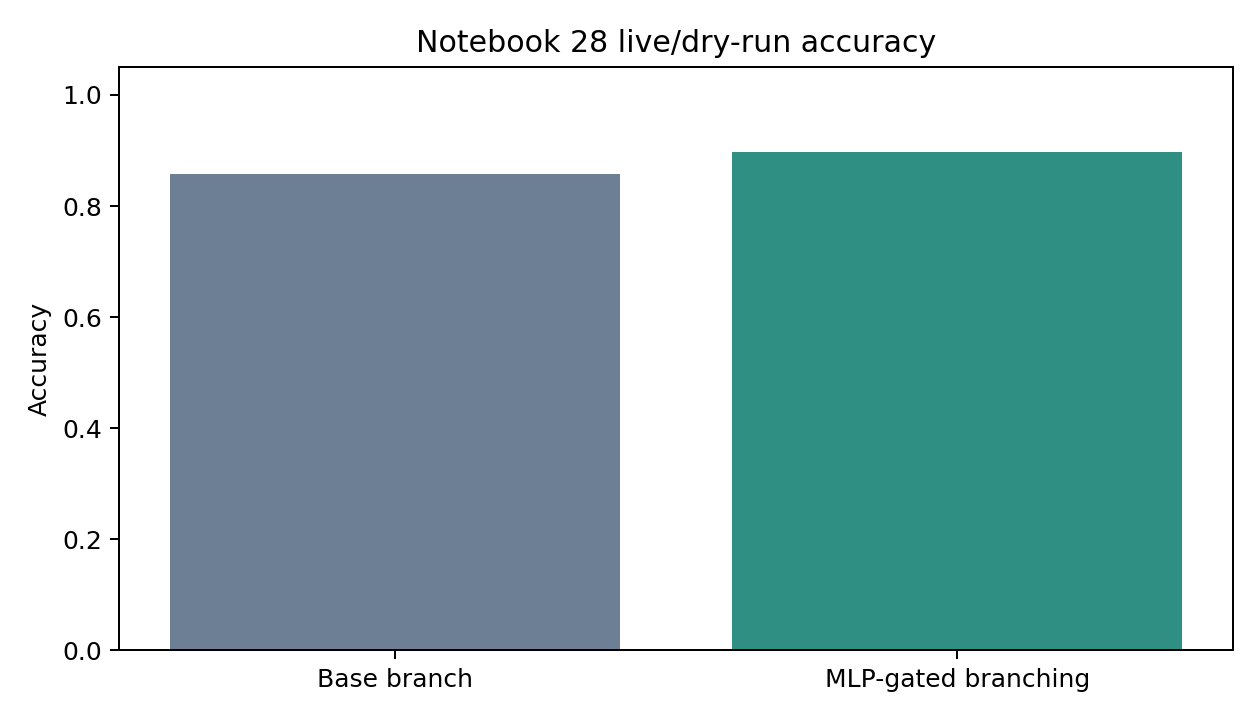
\includegraphics[width=\linewidth]{artifacts/trajectory_replicates/mlp_gated_confounder_graph_bayes_branching_49case_v1/figures/accuracy_comparison.png}
\caption{Notebook 28 accuracy comparison.}
\end{subfigure}
\hfill
\begin{subfigure}{0.48\linewidth}
\centering
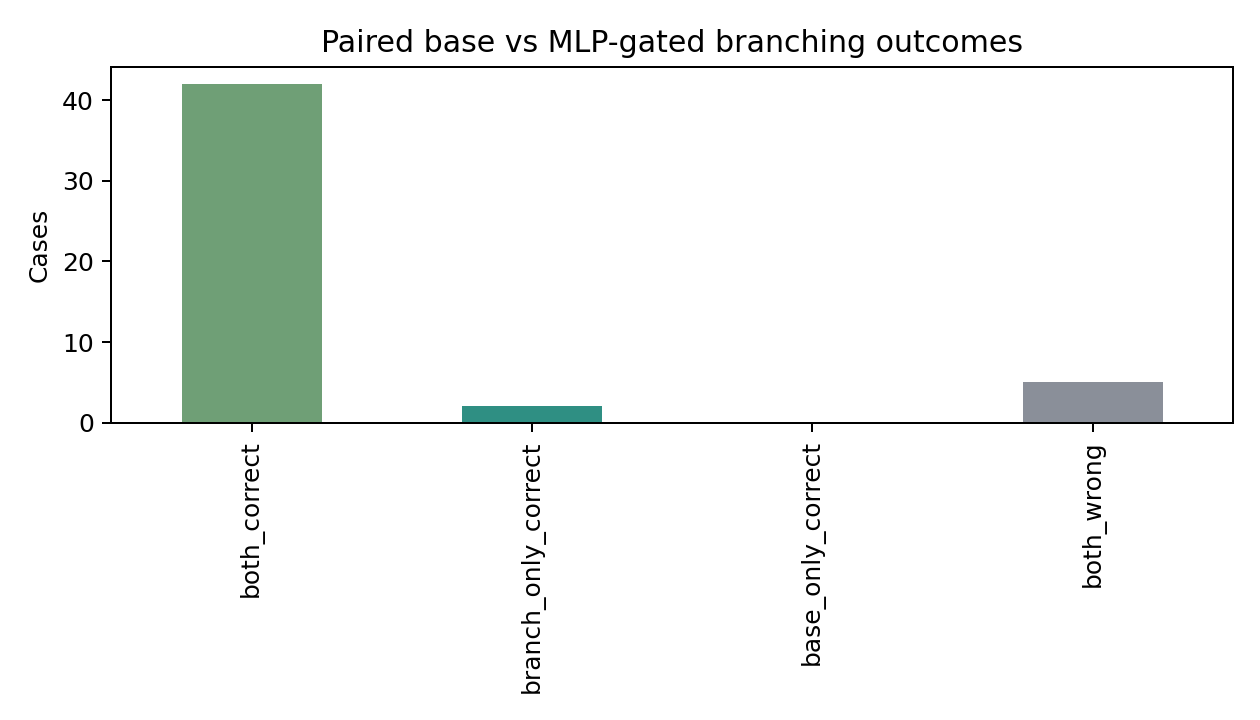
\includegraphics[width=\linewidth]{artifacts/trajectory_replicates/mlp_gated_confounder_graph_bayes_branching_49case_v1/figures/paired_outcomes.png}
\caption{Paired outcomes vs base.}
\end{subfigure}
\caption{Notebook 28 improves over its same-run base with zero regressions, but is not promoted as the final method.}
\end{figure}

\begin{figure}[H]
\centering
\begin{subfigure}{0.48\linewidth}
\centering
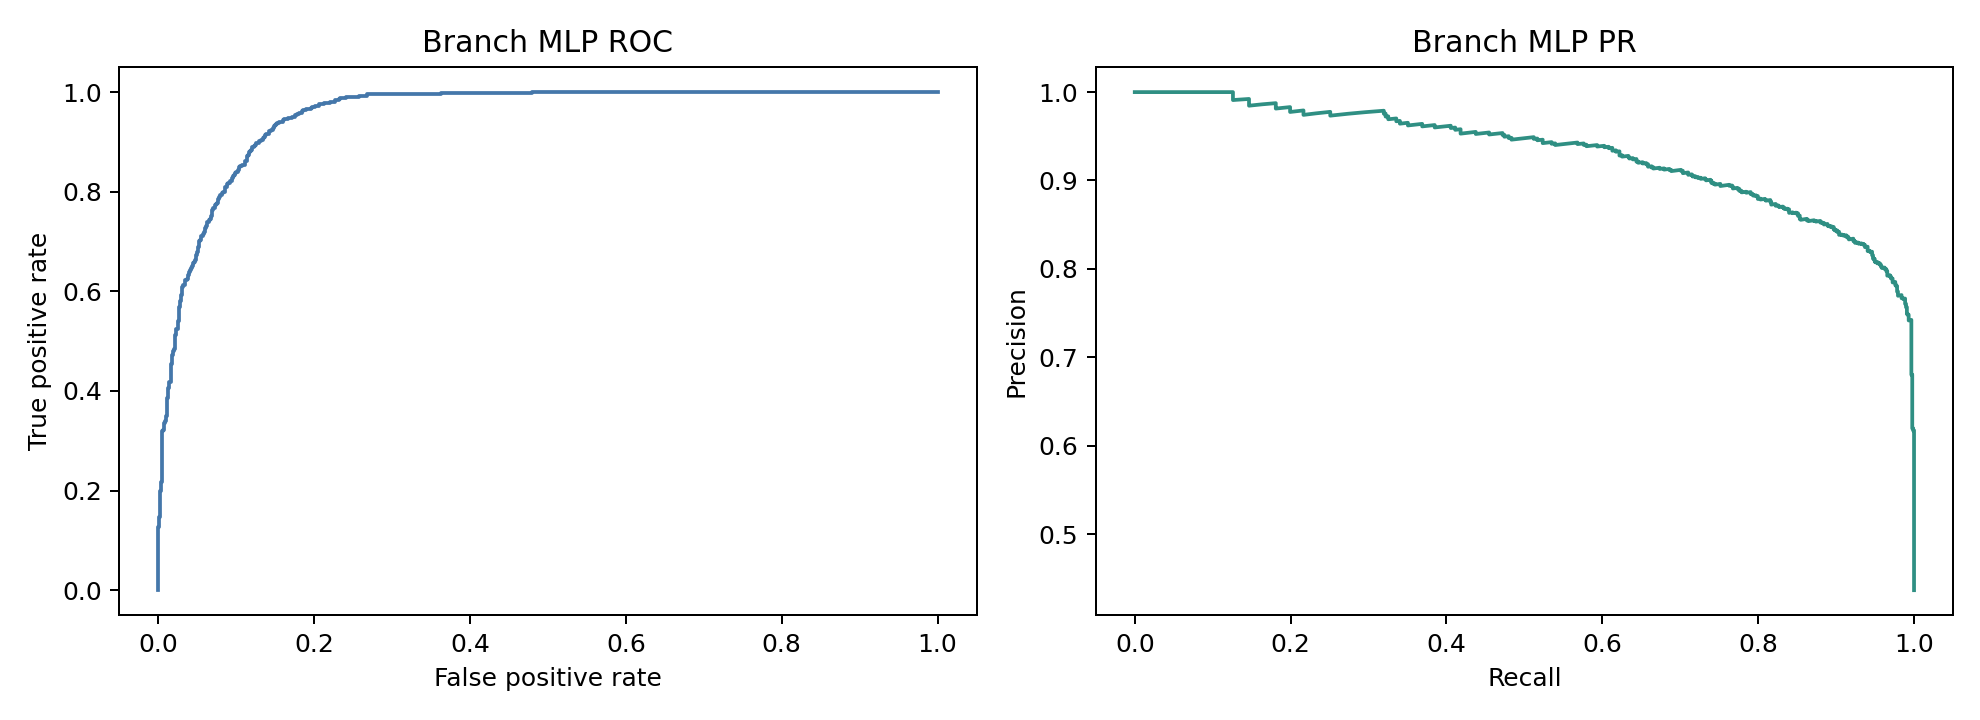
\includegraphics[width=\linewidth]{artifacts/trajectory_replicates/mlp_gated_confounder_graph_bayes_branching_49case_v1/figures/branch_mlp_roc_pr_curves.png}
\caption{Branch-trigger MLP ROC/PR.}
\end{subfigure}
\hfill
\begin{subfigure}{0.48\linewidth}
\centering
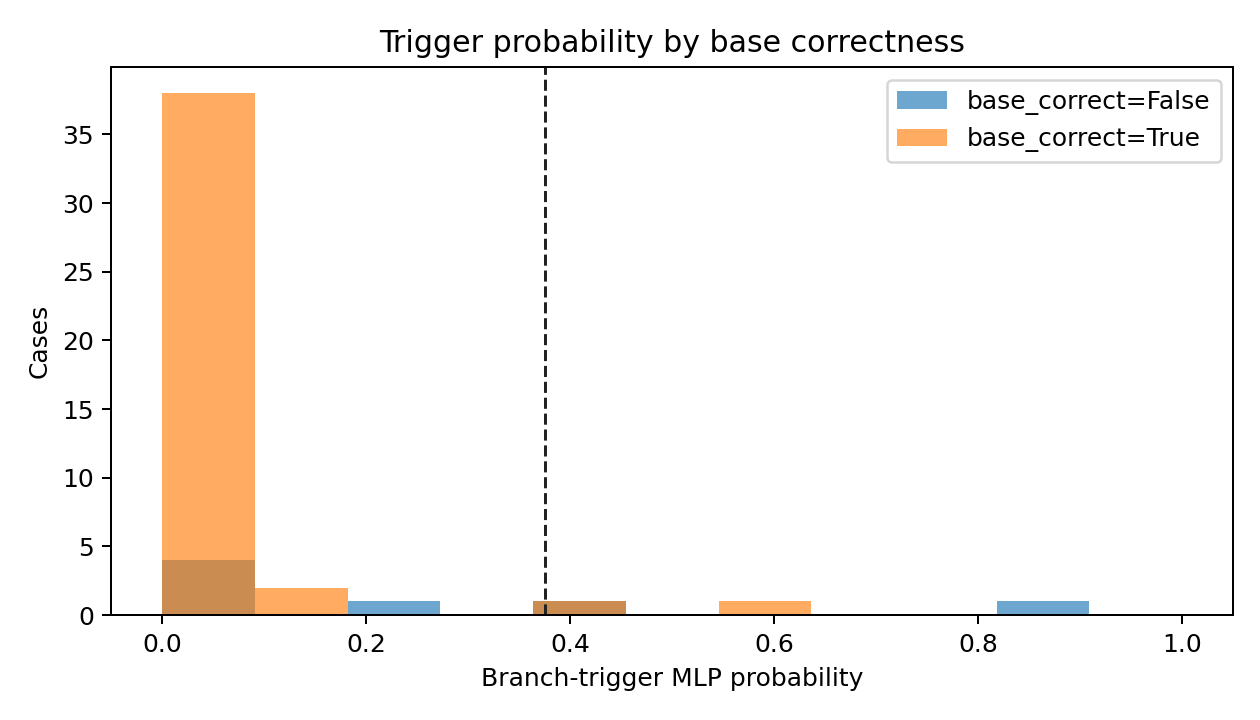
\includegraphics[width=\linewidth]{artifacts/trajectory_replicates/mlp_gated_confounder_graph_bayes_branching_49case_v1/figures/branch_trigger_probability_by_correctness.png}
\caption{Trigger probability by correctness.}
\end{subfigure}
\caption{Notebook 28 replaces hand-written branch suspicion with a learned gate over MLP, graph, Bayes, request-count, and confounder-coverage features.}
\end{figure}

\section{Error Analysis}

The early hard cases included Croup and Pericarditis. Later graph/Bayes work showed that Croup was recoverable by graph support, while Pericarditis remained difficult because the revealed evidence state often failed to support it strongly enough.

Notebook 13's original six misses were narrowed by the offline rescue layer. After Notebook 23 rescue, the remaining saved-trace misses were:
\begin{table}[H]
\centering
\caption{Remaining saved-trace errors after offline graph/Bayes rescue.}
\begin{tabular}{llll}
\toprule
Case & True pathology & Prediction & Stop pattern \\
\midrule
\texttt{test:111176} & Acute rhinosinusitis & Chronic rhinosinusitis & selected MLP stop \\
\texttt{test:62878} & Pericarditis & Anemia & agent stop \\
\bottomrule
\end{tabular}
\end{table}

The important failure pattern is wrong-belief convergence, not simply insufficient request budget. Some wrong cases use many requests and still settle on the wrong diagnosis. In other cases, the MLP becomes confident too early because the currently visible evidence strongly supports a nearby confounder.

Notebook 15 also shows that more evidence is not monotonically beneficial. Later evidence can cause correct-to-wrong drift, especially when it is generic or shifts attention toward a common confounder. This supports the ledger-stop design: the system should stop when enough discriminative evidence has been acquired, not when every possible field has been exhausted.

\begin{figure}[H]
\centering
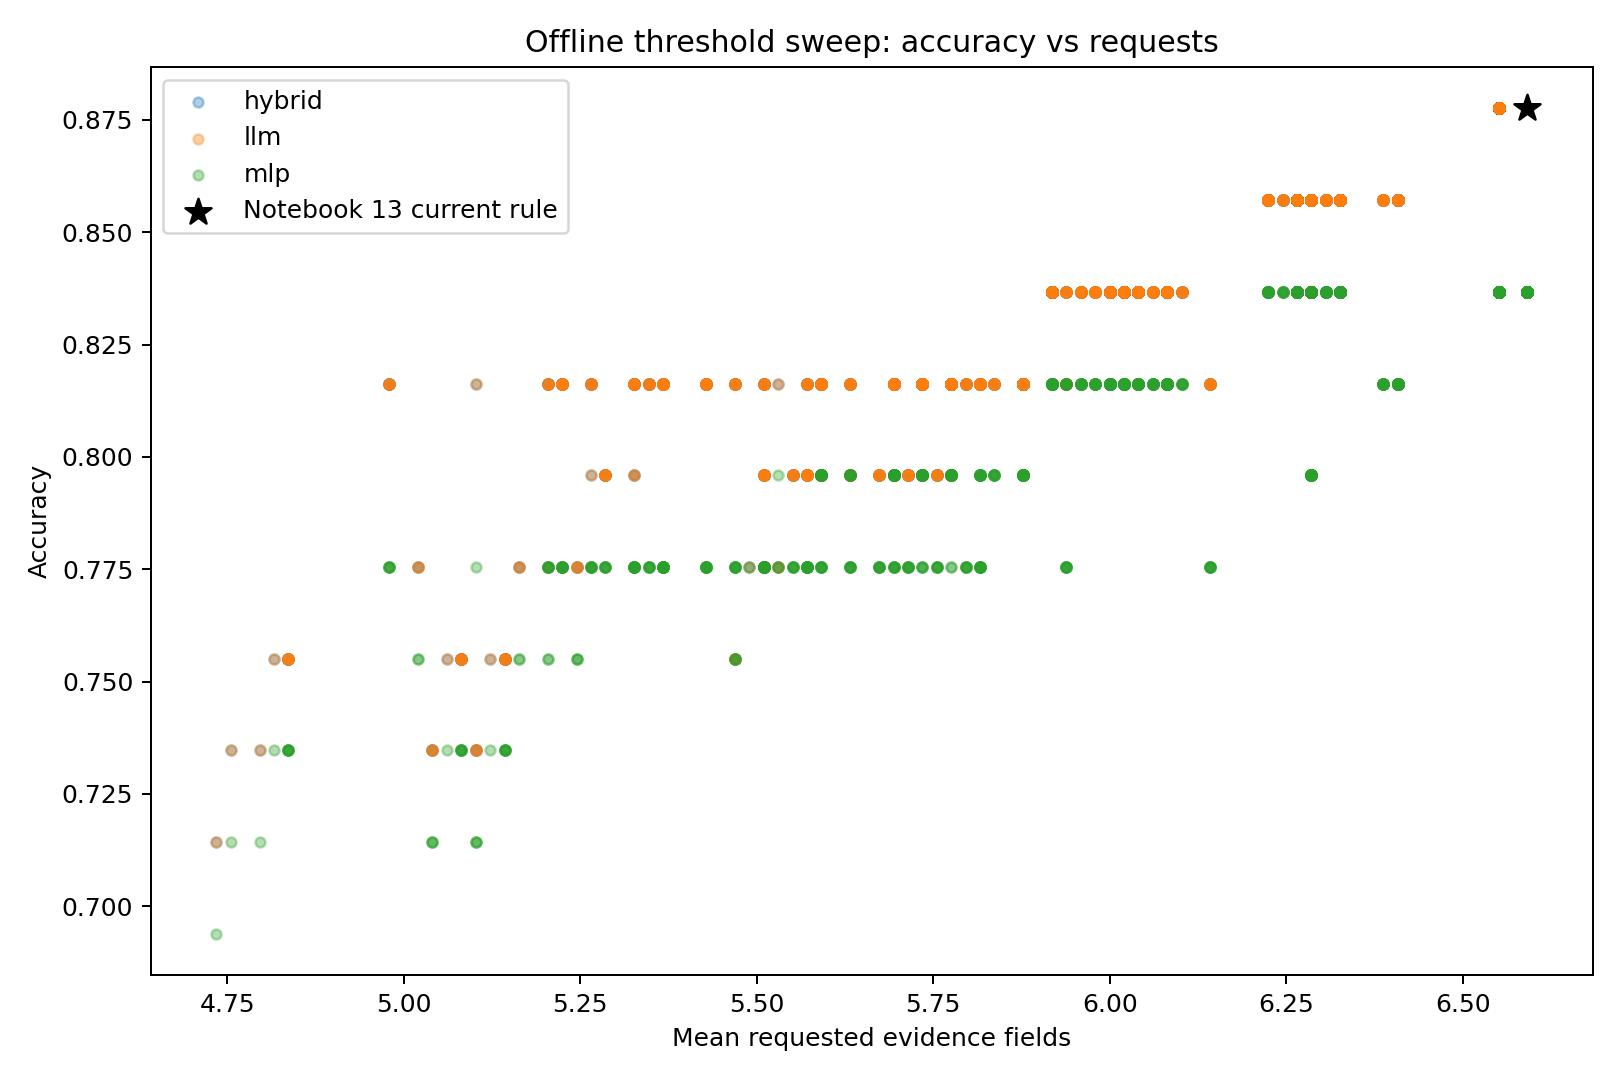
\includegraphics[width=0.82\linewidth]{artifacts/stop_policy_sensitivity/notebook13_49case_v1/figures/threshold_sweep_accuracy_vs_requests.png}
\caption{Stop-threshold sensitivity over the Notebook 13 49-case traces.}
\end{figure}

\section{Claims Supported and Not Supported}

\subsection{Supported Claims}

\begin{itemize}[leftmargin=*]
    \item A faithful \ddx{} deep-learning baseline was implemented using structured BASD-style evidence encoding.
    \item Initial evidence alone is insufficient for strong diagnosis: the full-test MLP reaches only $0.378$ accuracy.
    \item Full structured evidence is near-ceiling: the full-evidence MLP reaches $0.996$ accuracy.
    \item Sequential evidence acquisition substantially improves over initial-evidence diagnosis on balanced live slices.
    \item Online MLP-guided stopping improves evidence efficiency relative to pure LLM stopping at matched request budgets.
    \item The defended Notebook 13 live method reaches $43/49$ with $6.59$ mean evidence requests.
    \item A fresh Notebook 13-style live base run reaches $45/49$ with $6.20$ mean requests, supporting base-method robustness.
    \item Graph and Bayesian signals contain useful diagnostic information, especially for final-state critique and rescue analysis.
    \item Targeted branching can recover some locked-in wrong trajectories. Notebook 28 improves the same-run base from $42/49$ to $44/49$ with zero regressions by using a learned branch gate, pseudo-candidates, and base protection.
\end{itemize}

\subsection{Unsupported Claims}

\begin{itemize}[leftmargin=*]
    \item The project does not prove that multi-agent diagnosis is superior. Notebooks 27 and 28 are partial branching confirmations, not promoted final methods.
    \item The project does not prove the \llm{} final answer is generally better than a neural classifier.
    \item Direct MLP-guided question selection was tested and rejected.
    \item Hard graph top-10 question shortlisting was tested and rejected.
    \item Offline Bayesian VOI replacement control was tested and rejected.
    \item Offline graph/Bayes rescue should not be claimed as live-promoted; Notebook 24 did not confirm it as an improvement.
    \item Notebook 28 should not be claimed as the final promoted method; it improves its own base safely, but it reaches $44/49$, below the $47/49$ target and below the strongest fresh Notebook 13-style base run.
    \item The project does not claim clinical deployment readiness. \ddx{} is synthetic, and the live slices are balanced benchmark samples.
\end{itemize}

\section{Limitations}

The largest limitation is sample size for live \llm{} experiments. Full-test neural baselines use the official test split, but sequential \llm{} experiments are expensive and therefore use balanced 24-case and 49-case slices. A second limitation is that the partial-evidence \mlp{} is trained on policy-shaped masks; when a different controller creates different trajectories, as in Notebook 19, the \mlp{} may be out of distribution. A third limitation is that the graph and Bayesian rescue results are trace-dependent. They are valuable diagnostics, but fresh live confirmation shows that saved-trace rescue can overfit to a particular failure pattern.

The project also does not reproduce official \ddx{} RL baselines end to end. Instead, it builds a course-project baseline ladder and contextualizes against prior work. Any future claim of superiority over MEDDxAgent, AARLC, or MedKGI-style systems would require matched sampling, comparable question budgets, and consistent metrics.

\section{Future Work}

The most promising next direction is not majority-vote branching. The trajectory lab shows majority voting does not improve the 49-case result. Notebook 28 already implements the first learned version of the better direction: cautious selective branching with graph/Bayes/MLP pseudo-candidates, confounder coverage, and base protection. The remaining problem is not whether branching can help at all; it is whether branch triggering and resolver calibration can reach the offline $47/49$ opportunity without adding large request cost.

Specific next steps:
\begin{enumerate}[leftmargin=*]
    \item Improve the Notebook 28 branch-trigger classifier with more held-out live-style development traces rather than only synthetic partial states.
    \item Calibrate the graph/Bayes/MLP resolver so pseudo-candidates can fix silent consensus errors without overusing branches.
    \item Target known confounder clusters: acute versus chronic rhinosinusitis, COPD versus asthma, pediatric airway infections, and cardiac inflammatory syndromes.
    \item Expand live confirmation beyond 49 balanced cases.
    \item Reserve held-out development traces before learning any final graph adjudicator.
\end{enumerate}

\section{Conclusion}

This project produced a technically complete diagnostic workup system and a careful evidence trail. The strongest defended method is a ledger-controlled sequential \llm{} workup with online partial-evidence \mlp{} stopping. It improves dramatically over initial-evidence diagnosis and uses far fewer fields than full evidence. The project also honestly reports negative and partial results: direct MLP question control, hard graph shortlisting, Bayesian VOI replacement, live graph/Bayes rescue, Notebook 27 hand-triggered branching, and Notebook 28 learned branching are not promoted as final methods. These results make the final claim stronger, not weaker, because they show that the proposed architecture was selected through controlled ablation rather than optimistic storytelling.

The final defended statement is:
\begin{quote}
We built a reproducible \ddx{} baseline ladder and proposed a structured sequential workup system where an \llm{} acquires evidence under a deterministic ledger and a partial-evidence \mlp{} decides when enough information has been gathered. The frozen live 49-case confirmation reached $43/49$ accuracy and $0.939$ top-5 while requesting about $6.6$ evidence fields per case; a fresh live run of the same backbone reached $45/49$ with $6.20$ requests. Offline graph/Bayes enhancements and Notebook 28 learned branching are promising, but they are not promoted over the defended Notebook 13-style backbone.
\end{quote}

\newpage
\begin{thebibliography}{99}

\bibitem{ddxplus}
Tchango, A. F., Goel, R., Wen, Z., Martel, J., \& Ghosn, J.
\newblock \emph{DDXPlus: A New Dataset For Automatic Medical Diagnosis}.
\newblock NeurIPS Datasets and Benchmarks, 2022.

\bibitem{aarlc}
Xia, Y., Zhou, J., Shi, Z., et al.
\newblock \emph{Efficient Symptom Inquiring and Diagnosis via Adaptive Alignment of Reinforcement Learning and Classification}.
\newblock arXiv:2112.00733.

\bibitem{afa}
Ma, C., Tschiatschek, S., Palla, K., Hernandez-Lobato, J. M., Nowozin, S., \& Zhang, C.
\newblock \emph{Joint Active Feature Acquisition and Classification with Variable-Size Set Encoding}.
\newblock NeurIPS, 2018.

\bibitem{costsensitive}
Saar-Tsechansky, M., Melville, P., \& Provost, F.
\newblock \emph{Cost-sensitive feature acquisition and classification}.
\newblock Pattern Recognition, 2007.

\bibitem{ddxt}
\emph{DDxT: Deep Generative Transformer Models for Differential Diagnosis}.
\newblock arXiv:2312.01242.

\bibitem{meddxagent}
\emph{MEDDxAgent: A Unified Modular Agent Framework for Explainable Automatic Differential Diagnosis}.
\newblock arXiv:2502.19175.

\bibitem{mediq}
\emph{MediQ: Question-Asking LLMs and a Benchmark for Reliable Interactive Clinical Reasoning}.
\newblock arXiv:2406.00922.

\bibitem{alfa}
\emph{ALFA: Aligning LLMs to Ask Good Questions: A Case Study in Clinical Reasoning}.
\newblock arXiv:2502.14860.

\bibitem{kg4diagnosis}
\emph{KG4Diagnosis: A Hierarchical Multi-Agent LLM Framework with Knowledge Graph Enhancement for Medical Diagnosis}.
\newblock arXiv:2412.16833.

\bibitem{medrag}
\emph{MedRAG: Enhancing Retrieval-augmented Generation with Knowledge Graph-Elicited Reasoning for Healthcare Copilot}.
\newblock arXiv:2502.04413.

\bibitem{trimediq}
\emph{Triplet-Structured Knowledge Integration for Multi-Turn Medical Reasoning}.
\newblock arXiv:2510.03536.

\bibitem{medkgi}
\emph{MedKGI: Iterative Differential Diagnosis with Medical Knowledge Graphs and Information-Guided Inquiring}.
\newblock arXiv:2512.24181.

\bibitem{bayesinquiry}
\emph{A Bayesian Approach for Medical Inquiry and Disease Inference in Automated Differential Diagnosis}.
\newblock arXiv:2110.08393.

\bibitem{entropytest}
\emph{Efficient Test Selection in Active Diagnosis via Entropy Approximation}.
\newblock arXiv:1207.1418.

\end{thebibliography}

\end{document}
